% Options for packages loaded elsewhere
\PassOptionsToPackage{unicode}{hyperref}
\PassOptionsToPackage{hyphens}{url}
\PassOptionsToPackage{dvipsnames,svgnames,x11names}{xcolor}
%
\documentclass[
  letterpaper,
  DIV=11,
  numbers=noendperiod]{scrartcl}

\usepackage{amsmath,amssymb}
\usepackage{iftex}
\ifPDFTeX
  \usepackage[T1]{fontenc}
  \usepackage[utf8]{inputenc}
  \usepackage{textcomp} % provide euro and other symbols
\else % if luatex or xetex
  \usepackage{unicode-math}
  \defaultfontfeatures{Scale=MatchLowercase}
  \defaultfontfeatures[\rmfamily]{Ligatures=TeX,Scale=1}
\fi
\usepackage{lmodern}
\ifPDFTeX\else  
    % xetex/luatex font selection
\fi
% Use upquote if available, for straight quotes in verbatim environments
\IfFileExists{upquote.sty}{\usepackage{upquote}}{}
\IfFileExists{microtype.sty}{% use microtype if available
  \usepackage[]{microtype}
  \UseMicrotypeSet[protrusion]{basicmath} % disable protrusion for tt fonts
}{}
\makeatletter
\@ifundefined{KOMAClassName}{% if non-KOMA class
  \IfFileExists{parskip.sty}{%
    \usepackage{parskip}
  }{% else
    \setlength{\parindent}{0pt}
    \setlength{\parskip}{6pt plus 2pt minus 1pt}}
}{% if KOMA class
  \KOMAoptions{parskip=half}}
\makeatother
\usepackage{xcolor}
\setlength{\emergencystretch}{3em} % prevent overfull lines
\setcounter{secnumdepth}{-\maxdimen} % remove section numbering
% Make \paragraph and \subparagraph free-standing
\makeatletter
\ifx\paragraph\undefined\else
  \let\oldparagraph\paragraph
  \renewcommand{\paragraph}{
    \@ifstar
      \xxxParagraphStar
      \xxxParagraphNoStar
  }
  \newcommand{\xxxParagraphStar}[1]{\oldparagraph*{#1}\mbox{}}
  \newcommand{\xxxParagraphNoStar}[1]{\oldparagraph{#1}\mbox{}}
\fi
\ifx\subparagraph\undefined\else
  \let\oldsubparagraph\subparagraph
  \renewcommand{\subparagraph}{
    \@ifstar
      \xxxSubParagraphStar
      \xxxSubParagraphNoStar
  }
  \newcommand{\xxxSubParagraphStar}[1]{\oldsubparagraph*{#1}\mbox{}}
  \newcommand{\xxxSubParagraphNoStar}[1]{\oldsubparagraph{#1}\mbox{}}
\fi
\makeatother

\usepackage{color}
\usepackage{fancyvrb}
\newcommand{\VerbBar}{|}
\newcommand{\VERB}{\Verb[commandchars=\\\{\}]}
\DefineVerbatimEnvironment{Highlighting}{Verbatim}{commandchars=\\\{\}}
% Add ',fontsize=\small' for more characters per line
\usepackage{framed}
\definecolor{shadecolor}{RGB}{241,243,245}
\newenvironment{Shaded}{\begin{snugshade}}{\end{snugshade}}
\newcommand{\AlertTok}[1]{\textcolor[rgb]{0.68,0.00,0.00}{#1}}
\newcommand{\AnnotationTok}[1]{\textcolor[rgb]{0.37,0.37,0.37}{#1}}
\newcommand{\AttributeTok}[1]{\textcolor[rgb]{0.40,0.45,0.13}{#1}}
\newcommand{\BaseNTok}[1]{\textcolor[rgb]{0.68,0.00,0.00}{#1}}
\newcommand{\BuiltInTok}[1]{\textcolor[rgb]{0.00,0.23,0.31}{#1}}
\newcommand{\CharTok}[1]{\textcolor[rgb]{0.13,0.47,0.30}{#1}}
\newcommand{\CommentTok}[1]{\textcolor[rgb]{0.37,0.37,0.37}{#1}}
\newcommand{\CommentVarTok}[1]{\textcolor[rgb]{0.37,0.37,0.37}{\textit{#1}}}
\newcommand{\ConstantTok}[1]{\textcolor[rgb]{0.56,0.35,0.01}{#1}}
\newcommand{\ControlFlowTok}[1]{\textcolor[rgb]{0.00,0.23,0.31}{\textbf{#1}}}
\newcommand{\DataTypeTok}[1]{\textcolor[rgb]{0.68,0.00,0.00}{#1}}
\newcommand{\DecValTok}[1]{\textcolor[rgb]{0.68,0.00,0.00}{#1}}
\newcommand{\DocumentationTok}[1]{\textcolor[rgb]{0.37,0.37,0.37}{\textit{#1}}}
\newcommand{\ErrorTok}[1]{\textcolor[rgb]{0.68,0.00,0.00}{#1}}
\newcommand{\ExtensionTok}[1]{\textcolor[rgb]{0.00,0.23,0.31}{#1}}
\newcommand{\FloatTok}[1]{\textcolor[rgb]{0.68,0.00,0.00}{#1}}
\newcommand{\FunctionTok}[1]{\textcolor[rgb]{0.28,0.35,0.67}{#1}}
\newcommand{\ImportTok}[1]{\textcolor[rgb]{0.00,0.46,0.62}{#1}}
\newcommand{\InformationTok}[1]{\textcolor[rgb]{0.37,0.37,0.37}{#1}}
\newcommand{\KeywordTok}[1]{\textcolor[rgb]{0.00,0.23,0.31}{\textbf{#1}}}
\newcommand{\NormalTok}[1]{\textcolor[rgb]{0.00,0.23,0.31}{#1}}
\newcommand{\OperatorTok}[1]{\textcolor[rgb]{0.37,0.37,0.37}{#1}}
\newcommand{\OtherTok}[1]{\textcolor[rgb]{0.00,0.23,0.31}{#1}}
\newcommand{\PreprocessorTok}[1]{\textcolor[rgb]{0.68,0.00,0.00}{#1}}
\newcommand{\RegionMarkerTok}[1]{\textcolor[rgb]{0.00,0.23,0.31}{#1}}
\newcommand{\SpecialCharTok}[1]{\textcolor[rgb]{0.37,0.37,0.37}{#1}}
\newcommand{\SpecialStringTok}[1]{\textcolor[rgb]{0.13,0.47,0.30}{#1}}
\newcommand{\StringTok}[1]{\textcolor[rgb]{0.13,0.47,0.30}{#1}}
\newcommand{\VariableTok}[1]{\textcolor[rgb]{0.07,0.07,0.07}{#1}}
\newcommand{\VerbatimStringTok}[1]{\textcolor[rgb]{0.13,0.47,0.30}{#1}}
\newcommand{\WarningTok}[1]{\textcolor[rgb]{0.37,0.37,0.37}{\textit{#1}}}

\providecommand{\tightlist}{%
  \setlength{\itemsep}{0pt}\setlength{\parskip}{0pt}}\usepackage{longtable,booktabs,array}
\usepackage{calc} % for calculating minipage widths
% Correct order of tables after \paragraph or \subparagraph
\usepackage{etoolbox}
\makeatletter
\patchcmd\longtable{\par}{\if@noskipsec\mbox{}\fi\par}{}{}
\makeatother
% Allow footnotes in longtable head/foot
\IfFileExists{footnotehyper.sty}{\usepackage{footnotehyper}}{\usepackage{footnote}}
\makesavenoteenv{longtable}
\usepackage{graphicx}
\makeatletter
\def\maxwidth{\ifdim\Gin@nat@width>\linewidth\linewidth\else\Gin@nat@width\fi}
\def\maxheight{\ifdim\Gin@nat@height>\textheight\textheight\else\Gin@nat@height\fi}
\makeatother
% Scale images if necessary, so that they will not overflow the page
% margins by default, and it is still possible to overwrite the defaults
% using explicit options in \includegraphics[width, height, ...]{}
\setkeys{Gin}{width=\maxwidth,height=\maxheight,keepaspectratio}
% Set default figure placement to htbp
\makeatletter
\def\fps@figure{htbp}
\makeatother

\usepackage{fvextra}
\DefineVerbatimEnvironment{Highlighting}{Verbatim}{breaklines,commandchars=\\\{\}}
\KOMAoption{captions}{tableheading}
\makeatletter
\@ifpackageloaded{caption}{}{\usepackage{caption}}
\AtBeginDocument{%
\ifdefined\contentsname
  \renewcommand*\contentsname{Table of contents}
\else
  \newcommand\contentsname{Table of contents}
\fi
\ifdefined\listfigurename
  \renewcommand*\listfigurename{List of Figures}
\else
  \newcommand\listfigurename{List of Figures}
\fi
\ifdefined\listtablename
  \renewcommand*\listtablename{List of Tables}
\else
  \newcommand\listtablename{List of Tables}
\fi
\ifdefined\figurename
  \renewcommand*\figurename{Figure}
\else
  \newcommand\figurename{Figure}
\fi
\ifdefined\tablename
  \renewcommand*\tablename{Table}
\else
  \newcommand\tablename{Table}
\fi
}
\@ifpackageloaded{float}{}{\usepackage{float}}
\floatstyle{ruled}
\@ifundefined{c@chapter}{\newfloat{codelisting}{h}{lop}}{\newfloat{codelisting}{h}{lop}[chapter]}
\floatname{codelisting}{Listing}
\newcommand*\listoflistings{\listof{codelisting}{List of Listings}}
\makeatother
\makeatletter
\makeatother
\makeatletter
\@ifpackageloaded{caption}{}{\usepackage{caption}}
\@ifpackageloaded{subcaption}{}{\usepackage{subcaption}}
\makeatother

\ifLuaTeX
  \usepackage{selnolig}  % disable illegal ligatures
\fi
\usepackage{bookmark}

\IfFileExists{xurl.sty}{\usepackage{xurl}}{} % add URL line breaks if available
\urlstyle{same} % disable monospaced font for URLs
\hypersetup{
  pdftitle={Your Title},
  colorlinks=true,
  linkcolor={blue},
  filecolor={Maroon},
  citecolor={Blue},
  urlcolor={Blue},
  pdfcreator={LaTeX via pandoc}}


\title{Your Title}
\author{}
\date{}

\begin{document}
\maketitle

\RecustomVerbatimEnvironment{verbatim}{Verbatim}{
  showspaces = false,
  showtabs = false,
  breaksymbolleft={},
  breaklines
}


\textbf{PS4:} Due Sat Nov 2 at 5:00PM Central. Worth 100 points. We use
(\texttt{*}) to indicate a problem that we think might be time
consuming.

\subsection{Style Points (10 pts)}\label{style-points-10-pts}

Please refer to the minilesson on code style
\textbf{\href{https://uchicago.zoom.us/rec/share/pG_wQ-pHTQrJTmqNn4rcrw5V194M2H2s-2jdy8oVhWHkd_yZt9o162IWurpA-fxU.BIQlSgZLRYctvzp-}{here}}.

\subsection{Submission Steps (10 pts)}\label{submission-steps-10-pts}

\begin{enumerate}
\def\labelenumi{\arabic{enumi}.}
\tightlist
\item
  This problem set is a paired problem set.
\item
  Play paper, scissors, rock to determine who goes first. Call that
  person \emph{Partner 1}.

  \begin{itemize}
  \tightlist
  \item
    Partner 1 (name and cnet ID): Alejandra Silva - aosilva
  \item
    Partner 2 (name and cnet ID): Guillermina Marto - gmarto
  \end{itemize}
\item
  Partner 1 will accept the \texttt{ps4} and then share the link it
  creates with their partner. You can only share it with one partner so
  you will not be able to change it after your partner has accepted.
\item
  ``This submission is our work alone and complies with the 30538
  integrity policy.'' Add your initials to indicate your agreement:
  \textbf{AS} \textbf{GM}
\item
  ``I have uploaded the names of anyone else other than my partner and I
  worked with on the problem set
  \textbf{\href{https://docs.google.com/forms/d/185usrCREQaUbvAXpWhChkjghdGgmAZXA3lPWpXLLsts/edit}{here}}''
  (1 point)
\item
  Late coins used this pset: **\_\_** Late coins left after submission:
  **\_\_**
\item
  Knit your \texttt{ps4.qmd} to an PDF file to make \texttt{ps4.pdf},

  \begin{itemize}
  \tightlist
  \item
    The PDF should not be more than 25 pages. Use \texttt{head()} and
    re-size figures when appropriate.
  \end{itemize}
\item
  (Partner 1): push \texttt{ps4.qmd} and \texttt{ps4.pdf} to your github
  repo.
\item
  (Partner 1): submit \texttt{ps4.pdf} via Gradescope. Add your partner
  on Gradescope.
\item
  (Partner 1): tag your submission in Gradescope
\end{enumerate}

\textbf{Important:} Repositories are for tracking code. \textbf{Do not
commit the data or shapefiles to your repo.} The best way to do this is
with \texttt{.gitignore}, which we have covered in class. If you do
accidentally commit the data, Github has a
\href{https://docs.github.com/en/repositories/working-with-files/managing-large-files/about-large-files-on-github\#removing-files-from-a-repositorys-history}{guide}.
The best course of action depends on whether you have pushed yet. This
also means that both partners will have to download the initial raw data
and any data cleaning code will need to be re-run on both partners'
computers.

\subsection{Download and explore the Provider of Services (POS) file (10
pts)}\label{download-and-explore-the-provider-of-services-pos-file-10-pts}

\begin{enumerate}
\def\labelenumi{\arabic{enumi}.}
\tightlist
\item
\end{enumerate}

\begin{Shaded}
\begin{Highlighting}[]
\ImportTok{import}\NormalTok{ requests}
\ImportTok{import}\NormalTok{ pandas }\ImportTok{as}\NormalTok{ pd}
\ImportTok{import}\NormalTok{ altair }\ImportTok{as}\NormalTok{ alt}

\NormalTok{base\_url }\OperatorTok{=} \StringTok{"https://data.cms.gov/data{-}api/v1/dataset/}\SpecialCharTok{\{uuid\}}\StringTok{/data"}
\NormalTok{uuid }\OperatorTok{=} \StringTok{"96ba2257{-}2080{-}49c1{-}9e5b{-}7726f9f83cad"}

\NormalTok{columns }\OperatorTok{=}\NormalTok{ [}
    \StringTok{"PRVDR\_CTGRY\_CD"}\NormalTok{,        }\CommentTok{\# Provider Category Code}
    \StringTok{"PRVDR\_CTGRY\_SBTYP\_CD"}\NormalTok{,  }\CommentTok{\# Provider Subtype Code}
    \StringTok{"PRVDR\_NUM"}\NormalTok{,             }\CommentTok{\# CMS Certification Number}
    \StringTok{"PGM\_TRMNTN\_CD"}\NormalTok{,         }\CommentTok{\# Termination Code}
    \StringTok{"FAC\_NAME"}\NormalTok{,              }\CommentTok{\# Facility Name}
    \StringTok{"ZIP\_CD"}\NormalTok{,                }\CommentTok{\# ZIP Code}
    \StringTok{"STATE\_CD"}               \CommentTok{\# State Abbreviation}
\NormalTok{]}

\NormalTok{columns\_param }\OperatorTok{=} \StringTok{","}\NormalTok{.join(columns)}

\NormalTok{offset }\OperatorTok{=} \DecValTok{0}
\NormalTok{limit }\OperatorTok{=} \DecValTok{5000}  \CommentTok{\#  API allows size to be set to 5000}

\NormalTok{all\_data }\OperatorTok{=}\NormalTok{ []}

\ControlFlowTok{while} \VariableTok{True}\NormalTok{:}
\NormalTok{    params }\OperatorTok{=}\NormalTok{ \{}

        \StringTok{"column"}\NormalTok{: columns\_param,}
        \StringTok{"size"}\NormalTok{: limit,}
        \StringTok{"offset"}\NormalTok{: offset}
\NormalTok{    \}}

\NormalTok{    url }\OperatorTok{=}\NormalTok{ base\_url.}\BuiltInTok{format}\NormalTok{(uuid}\OperatorTok{=}\NormalTok{uuid)}
\NormalTok{    response }\OperatorTok{=}\NormalTok{ requests.get(url, params}\OperatorTok{=}\NormalTok{params)}

    \ControlFlowTok{if}\NormalTok{ response.status\_code }\OperatorTok{!=} \DecValTok{200}\NormalTok{:}
        \BuiltInTok{print}\NormalTok{(}\SpecialStringTok{f"Error: }\SpecialCharTok{\{}\NormalTok{response}\SpecialCharTok{.}\NormalTok{status\_code}\SpecialCharTok{\}}\SpecialStringTok{, }\SpecialCharTok{\{}\NormalTok{response}\SpecialCharTok{.}\NormalTok{text}\SpecialCharTok{\}}\SpecialStringTok{"}\NormalTok{)}
        \ControlFlowTok{break}

\NormalTok{    data }\OperatorTok{=}\NormalTok{ response.json()}

    \ControlFlowTok{if} \KeywordTok{not}\NormalTok{ data:}
        \BuiltInTok{print}\NormalTok{(}\StringTok{"No more data available."}\NormalTok{)}
        \ControlFlowTok{break}

\NormalTok{    all\_data.extend(data)}

\NormalTok{    offset }\OperatorTok{+=}\NormalTok{ limit}
    \BuiltInTok{print}\NormalTok{(}\SpecialStringTok{f"Fetched }\SpecialCharTok{\{}\BuiltInTok{len}\NormalTok{(data)}\SpecialCharTok{\}}\SpecialStringTok{ rows, moving to next batch..."}\NormalTok{)}

\NormalTok{df }\OperatorTok{=}\NormalTok{ pd.DataFrame(all\_data)}


\NormalTok{df.to\_csv(}\StringTok{"pos2016.csv"}\NormalTok{, index}\OperatorTok{=}\VariableTok{False}\NormalTok{)}
\end{Highlighting}
\end{Shaded}

\begin{verbatim}
Fetched 5000 rows, moving to next batch...
Fetched 5000 rows, moving to next batch...
Fetched 5000 rows, moving to next batch...
Fetched 5000 rows, moving to next batch...
Fetched 5000 rows, moving to next batch...
Fetched 5000 rows, moving to next batch...
Fetched 5000 rows, moving to next batch...
Fetched 5000 rows, moving to next batch...
Fetched 5000 rows, moving to next batch...
Fetched 5000 rows, moving to next batch...
Fetched 5000 rows, moving to next batch...
Fetched 5000 rows, moving to next batch...
Fetched 5000 rows, moving to next batch...
Fetched 5000 rows, moving to next batch...
Fetched 5000 rows, moving to next batch...
Fetched 5000 rows, moving to next batch...
Fetched 5000 rows, moving to next batch...
Fetched 5000 rows, moving to next batch...
Fetched 5000 rows, moving to next batch...
Fetched 5000 rows, moving to next batch...
Fetched 5000 rows, moving to next batch...
Fetched 5000 rows, moving to next batch...
Fetched 5000 rows, moving to next batch...
Fetched 5000 rows, moving to next batch...
Fetched 5000 rows, moving to next batch...
Fetched 5000 rows, moving to next batch...
Fetched 5000 rows, moving to next batch...
Fetched 5000 rows, moving to next batch...
Fetched 1557 rows, moving to next batch...
No more data available.
\end{verbatim}

\begin{enumerate}
\def\labelenumi{\arabic{enumi}.}
\setcounter{enumi}{1}
\tightlist
\item
\end{enumerate}

\begin{Shaded}
\begin{Highlighting}[]
\NormalTok{df }\OperatorTok{=}\NormalTok{ pd.read\_csv(}\StringTok{"pos2016.csv"}\NormalTok{)}


\NormalTok{df\_st\_hospitals }\OperatorTok{=}\NormalTok{ df[}
\NormalTok{    (df[}\StringTok{"PRVDR\_CTGRY\_CD"}\NormalTok{] }\OperatorTok{==} \DecValTok{1}\NormalTok{) }\OperatorTok{\&} 
\NormalTok{    (df[}\StringTok{"PRVDR\_CTGRY\_SBTYP\_CD"}\NormalTok{] }\OperatorTok{==} \DecValTok{1}\NormalTok{)}
\NormalTok{]}

\NormalTok{num\_hospitals }\OperatorTok{=}\NormalTok{ df\_st\_hospitals.shape[}\DecValTok{0}\NormalTok{]}
\BuiltInTok{print}\NormalTok{(}\SpecialStringTok{f"Number of short{-}term hospitals reported in the data: }\SpecialCharTok{\{}\NormalTok{num\_hospitals}\SpecialCharTok{\}}\SpecialStringTok{"}\NormalTok{)}

\BuiltInTok{print}\NormalTok{(df\_st\_hospitals)}
\end{Highlighting}
\end{Shaded}

\begin{verbatim}
Number of short-term hospitals reported in the data: 7245
        PRVDR_CTGRY_CD  PRVDR_CTGRY_SBTYP_CD PRVDR_NUM  PGM_TRMNTN_CD  \
0                    1                   1.0    010001              0   
1                    1                   1.0    010004              1   
2                    1                   1.0    010005              0   
3                    1                   1.0    010006              0   
4                    1                   1.0    010007              0   
...                ...                   ...       ...            ...   
133526               1                   1.0    670114              0   
133527               1                   1.0    670115              0   
133528               1                   1.0    670116              0   
133529               1                   1.0    670117              0   
133530               1                   1.0    670118              0   

                                FAC_NAME   ZIP_CD STATE_CD  
0       SOUTHEAST ALABAMA MEDICAL CENTER  36301.0       AL  
1                 NORTH JACKSON HOSPITAL  35740.0       AL  
2          MARSHALL MEDICAL CENTER SOUTH  35957.0       AL  
3         ELIZA COFFEE MEMORIAL HOSPITAL  35631.0       AL  
4               MIZELL MEMORIAL HOSPITAL  36467.0       AL  
...                                  ...      ...      ...  
133526             WEIMAR MEDICAL CENTER  78962.0       TX  
133527      CLEVELAND EMERGENCY HOSPTIAL  77327.0       TX  
133528                WISE HEALTH SYSTEM  76177.0       TX  
133529  TEXAS GENERAL HOSPITAL- VZRMC LP  75140.0       TX  
133530              FIRST TEXAS HOSPITAL  77070.0       TX  

[7245 rows x 7 columns]
\end{verbatim}

The number of short-term hospitals reported in the dataset for Q4 2016
is 7,245.

According to the American Hospital Association (AHA) Annual Survey, the
estimated number of short-term hospitals is 4,500--5,000. Similarly, the
CMS Hospital Compare dataset indicates around 4,800 hospitals.

The discrepancy could be due to the narrower definition used in our
dataset and the timing of data collection, which only includes hospitals
in Q4 2016. Additionally, the CMS dataset might not include hospitals
that do not participate in Medicare or Medicaid, which could lead to
lower numbers.

\begin{enumerate}
\def\labelenumi{\arabic{enumi}.}
\setcounter{enumi}{2}
\tightlist
\item
\end{enumerate}

\begin{Shaded}
\begin{Highlighting}[]
\NormalTok{uuid\_dict }\OperatorTok{=}\NormalTok{ \{}
    \StringTok{"2016Q4"}\NormalTok{: }\StringTok{"96ba2257{-}2080{-}49c1{-}9e5b{-}7726f9f83cad"}\NormalTok{,}
    \StringTok{"2017Q4"}\NormalTok{: }\StringTok{"d338dc0d{-}641c{-}486a{-}b586{-}88a662f36963"}\NormalTok{,}
    \StringTok{"2018Q4"}\NormalTok{: }\StringTok{"4ff7fcfb{-}2a40{-}4f76{-}875d{-}a4ac2aec268e"}\NormalTok{,}
    \StringTok{"2019Q4"}\NormalTok{: }\StringTok{"03cca0cc{-}13a0{-}4b8d{-}82c4{-}57185b6bbfbd"}
\NormalTok{\}}

\NormalTok{columns }\OperatorTok{=}\NormalTok{ [}
    \StringTok{"PRVDR\_CTGRY\_CD"}\NormalTok{,        }\CommentTok{\# Provider Category Code}
    \StringTok{"PRVDR\_CTGRY\_SBTYP\_CD"}\NormalTok{,  }\CommentTok{\# Provider Subtype Code}
    \StringTok{"PRVDR\_NUM"}\NormalTok{,             }\CommentTok{\# CMS Certification Number}
    \StringTok{"PGM\_TRMNTN\_CD"}\NormalTok{,         }\CommentTok{\# Termination Code}
    \StringTok{"FAC\_NAME"}\NormalTok{,              }\CommentTok{\# Facility Name}
    \StringTok{"ZIP\_CD"}\NormalTok{,                }\CommentTok{\# ZIP Code}
    \StringTok{"STATE\_CD"}               \CommentTok{\# State Abbreviation}
\NormalTok{]}

\NormalTok{columns\_param }\OperatorTok{=} \StringTok{","}\NormalTok{.join(columns)}

\NormalTok{combined\_data }\OperatorTok{=}\NormalTok{ []}

\ControlFlowTok{for}\NormalTok{ year\_quarter, uuid }\KeywordTok{in}\NormalTok{ uuid\_dict.items():}
\NormalTok{    offset }\OperatorTok{=} \DecValTok{0}
\NormalTok{    limit }\OperatorTok{=} \DecValTok{5000}  
\NormalTok{    all\_data }\OperatorTok{=}\NormalTok{ []}

    \BuiltInTok{print}\NormalTok{(}\SpecialStringTok{f"Fetching data for }\SpecialCharTok{\{}\NormalTok{year\_quarter}\SpecialCharTok{\}}\SpecialStringTok{..."}\NormalTok{)}

    \ControlFlowTok{while} \VariableTok{True}\NormalTok{:}
\NormalTok{        params }\OperatorTok{=}\NormalTok{ \{}
            \StringTok{"column"}\NormalTok{: columns\_param,}
            \StringTok{"size"}\NormalTok{: limit,}
            \StringTok{"offset"}\NormalTok{: offset}
\NormalTok{        \}}

\NormalTok{        url }\OperatorTok{=} \SpecialStringTok{f"https://data.cms.gov/data{-}api/v1/dataset/}\SpecialCharTok{\{}\NormalTok{uuid}\SpecialCharTok{\}}\SpecialStringTok{/data"}
\NormalTok{        response }\OperatorTok{=}\NormalTok{ requests.get(url, params}\OperatorTok{=}\NormalTok{params)}

        \ControlFlowTok{if}\NormalTok{ response.status\_code }\OperatorTok{!=} \DecValTok{200}\NormalTok{:}
            \BuiltInTok{print}\NormalTok{(}\SpecialStringTok{f"Error: }\SpecialCharTok{\{}\NormalTok{response}\SpecialCharTok{.}\NormalTok{status\_code}\SpecialCharTok{\}}\SpecialStringTok{, }\SpecialCharTok{\{}\NormalTok{response}\SpecialCharTok{.}\NormalTok{text}\SpecialCharTok{\}}\SpecialStringTok{"}\NormalTok{)}
            \ControlFlowTok{break}

\NormalTok{        data }\OperatorTok{=}\NormalTok{ response.json()}

        \ControlFlowTok{if} \KeywordTok{not}\NormalTok{ data:}
            \BuiltInTok{print}\NormalTok{(}\StringTok{"No more data available."}\NormalTok{)}
            \ControlFlowTok{break}

\NormalTok{        all\_data.extend(data)}

\NormalTok{        offset }\OperatorTok{+=}\NormalTok{ limit}
        \BuiltInTok{print}\NormalTok{(}\SpecialStringTok{f"Fetched }\SpecialCharTok{\{}\BuiltInTok{len}\NormalTok{(data)}\SpecialCharTok{\}}\SpecialStringTok{ rows for }\SpecialCharTok{\{}\NormalTok{year\_quarter}\SpecialCharTok{\}}\SpecialStringTok{, moving to next batch..."}\NormalTok{)}

\NormalTok{    year\_data }\OperatorTok{=}\NormalTok{ pd.DataFrame(all\_data)}
\NormalTok{    year\_data[}\StringTok{"Year"}\NormalTok{] }\OperatorTok{=}\NormalTok{ year\_quarter[:}\DecValTok{4}\NormalTok{]}

    \CommentTok{\# filtro por las condiciones}
\NormalTok{    year\_data }\OperatorTok{=}\NormalTok{ year\_data[}
\NormalTok{    (year\_data[}\StringTok{"PRVDR\_CTGRY\_CD"}\NormalTok{] }\OperatorTok{==} \StringTok{"01"}\NormalTok{) }\OperatorTok{\&} 
\NormalTok{    (year\_data[}\StringTok{"PRVDR\_CTGRY\_SBTYP\_CD"}\NormalTok{] }\OperatorTok{==} \StringTok{"01"}\NormalTok{)}
\NormalTok{]  }

\NormalTok{    combined\_data.append(year\_data)}

\NormalTok{combined\_df }\OperatorTok{=}\NormalTok{ pd.concat(combined\_data, axis}\OperatorTok{=}\DecValTok{0}\NormalTok{)}

\NormalTok{combined\_df.to\_csv(}\StringTok{"combined\_data.csv"}\NormalTok{, index}\OperatorTok{=}\VariableTok{False}\NormalTok{)}

\BuiltInTok{print}\NormalTok{(}\SpecialStringTok{f"Total records retrieved across all years: }\SpecialCharTok{\{}\NormalTok{combined\_df}\SpecialCharTok{.}\NormalTok{shape[}\DecValTok{0}\NormalTok{]}\SpecialCharTok{\}}\SpecialStringTok{"}\NormalTok{)}
\end{Highlighting}
\end{Shaded}

\begin{verbatim}
Fetching data for 2016Q4...
Fetched 5000 rows for 2016Q4, moving to next batch...
Fetched 5000 rows for 2016Q4, moving to next batch...
Fetched 5000 rows for 2016Q4, moving to next batch...
Fetched 5000 rows for 2016Q4, moving to next batch...
Fetched 5000 rows for 2016Q4, moving to next batch...
Fetched 5000 rows for 2016Q4, moving to next batch...
Fetched 5000 rows for 2016Q4, moving to next batch...
Fetched 5000 rows for 2016Q4, moving to next batch...
Fetched 5000 rows for 2016Q4, moving to next batch...
Fetched 5000 rows for 2016Q4, moving to next batch...
Fetched 5000 rows for 2016Q4, moving to next batch...
Fetched 5000 rows for 2016Q4, moving to next batch...
Fetched 5000 rows for 2016Q4, moving to next batch...
Fetched 5000 rows for 2016Q4, moving to next batch...
Fetched 5000 rows for 2016Q4, moving to next batch...
Fetched 5000 rows for 2016Q4, moving to next batch...
Fetched 5000 rows for 2016Q4, moving to next batch...
Fetched 5000 rows for 2016Q4, moving to next batch...
Fetched 5000 rows for 2016Q4, moving to next batch...
Fetched 5000 rows for 2016Q4, moving to next batch...
Fetched 5000 rows for 2016Q4, moving to next batch...
Fetched 5000 rows for 2016Q4, moving to next batch...
Fetched 5000 rows for 2016Q4, moving to next batch...
Fetched 5000 rows for 2016Q4, moving to next batch...
Fetched 5000 rows for 2016Q4, moving to next batch...
Fetched 5000 rows for 2016Q4, moving to next batch...
Fetched 5000 rows for 2016Q4, moving to next batch...
Fetched 5000 rows for 2016Q4, moving to next batch...
Fetched 1557 rows for 2016Q4, moving to next batch...
No more data available.
Fetching data for 2017Q4...
Fetched 5000 rows for 2017Q4, moving to next batch...
Fetched 5000 rows for 2017Q4, moving to next batch...
Fetched 5000 rows for 2017Q4, moving to next batch...
Fetched 5000 rows for 2017Q4, moving to next batch...
Fetched 5000 rows for 2017Q4, moving to next batch...
Fetched 5000 rows for 2017Q4, moving to next batch...
Fetched 5000 rows for 2017Q4, moving to next batch...
Fetched 5000 rows for 2017Q4, moving to next batch...
Fetched 5000 rows for 2017Q4, moving to next batch...
Fetched 5000 rows for 2017Q4, moving to next batch...
Fetched 5000 rows for 2017Q4, moving to next batch...
Fetched 5000 rows for 2017Q4, moving to next batch...
Fetched 5000 rows for 2017Q4, moving to next batch...
Fetched 5000 rows for 2017Q4, moving to next batch...
Fetched 5000 rows for 2017Q4, moving to next batch...
Fetched 5000 rows for 2017Q4, moving to next batch...
Fetched 5000 rows for 2017Q4, moving to next batch...
Fetched 5000 rows for 2017Q4, moving to next batch...
Fetched 5000 rows for 2017Q4, moving to next batch...
Fetched 5000 rows for 2017Q4, moving to next batch...
Fetched 5000 rows for 2017Q4, moving to next batch...
Fetched 5000 rows for 2017Q4, moving to next batch...
Fetched 5000 rows for 2017Q4, moving to next batch...
Fetched 5000 rows for 2017Q4, moving to next batch...
Fetched 5000 rows for 2017Q4, moving to next batch...
Fetched 5000 rows for 2017Q4, moving to next batch...
Fetched 5000 rows for 2017Q4, moving to next batch...
Fetched 5000 rows for 2017Q4, moving to next batch...
Fetched 4110 rows for 2017Q4, moving to next batch...
No more data available.
Fetching data for 2018Q4...
Fetched 5000 rows for 2018Q4, moving to next batch...
Fetched 5000 rows for 2018Q4, moving to next batch...
Fetched 5000 rows for 2018Q4, moving to next batch...
Fetched 5000 rows for 2018Q4, moving to next batch...
Fetched 5000 rows for 2018Q4, moving to next batch...
Fetched 5000 rows for 2018Q4, moving to next batch...
Fetched 5000 rows for 2018Q4, moving to next batch...
Fetched 5000 rows for 2018Q4, moving to next batch...
Fetched 5000 rows for 2018Q4, moving to next batch...
Fetched 5000 rows for 2018Q4, moving to next batch...
Fetched 5000 rows for 2018Q4, moving to next batch...
Fetched 5000 rows for 2018Q4, moving to next batch...
Fetched 5000 rows for 2018Q4, moving to next batch...
Fetched 5000 rows for 2018Q4, moving to next batch...
Fetched 5000 rows for 2018Q4, moving to next batch...
Fetched 5000 rows for 2018Q4, moving to next batch...
Fetched 5000 rows for 2018Q4, moving to next batch...
Fetched 5000 rows for 2018Q4, moving to next batch...
Fetched 5000 rows for 2018Q4, moving to next batch...
Fetched 5000 rows for 2018Q4, moving to next batch...
Fetched 5000 rows for 2018Q4, moving to next batch...
Fetched 5000 rows for 2018Q4, moving to next batch...
Fetched 5000 rows for 2018Q4, moving to next batch...
Fetched 5000 rows for 2018Q4, moving to next batch...
Fetched 5000 rows for 2018Q4, moving to next batch...
Fetched 5000 rows for 2018Q4, moving to next batch...
Fetched 5000 rows for 2018Q4, moving to next batch...
Fetched 5000 rows for 2018Q4, moving to next batch...
Fetched 5000 rows for 2018Q4, moving to next batch...
Fetched 1696 rows for 2018Q4, moving to next batch...
No more data available.
Fetching data for 2019Q4...
Fetched 5000 rows for 2019Q4, moving to next batch...
Fetched 5000 rows for 2019Q4, moving to next batch...
Fetched 5000 rows for 2019Q4, moving to next batch...
Fetched 5000 rows for 2019Q4, moving to next batch...
Fetched 5000 rows for 2019Q4, moving to next batch...
Fetched 5000 rows for 2019Q4, moving to next batch...
Fetched 5000 rows for 2019Q4, moving to next batch...
Fetched 5000 rows for 2019Q4, moving to next batch...
Fetched 5000 rows for 2019Q4, moving to next batch...
Fetched 5000 rows for 2019Q4, moving to next batch...
Fetched 5000 rows for 2019Q4, moving to next batch...
Fetched 5000 rows for 2019Q4, moving to next batch...
Fetched 5000 rows for 2019Q4, moving to next batch...
Fetched 5000 rows for 2019Q4, moving to next batch...
Fetched 5000 rows for 2019Q4, moving to next batch...
Fetched 5000 rows for 2019Q4, moving to next batch...
Fetched 5000 rows for 2019Q4, moving to next batch...
Fetched 5000 rows for 2019Q4, moving to next batch...
Fetched 5000 rows for 2019Q4, moving to next batch...
Fetched 5000 rows for 2019Q4, moving to next batch...
Fetched 5000 rows for 2019Q4, moving to next batch...
Fetched 5000 rows for 2019Q4, moving to next batch...
Fetched 5000 rows for 2019Q4, moving to next batch...
Fetched 5000 rows for 2019Q4, moving to next batch...
Fetched 5000 rows for 2019Q4, moving to next batch...
Fetched 5000 rows for 2019Q4, moving to next batch...
Fetched 5000 rows for 2019Q4, moving to next batch...
Fetched 5000 rows for 2019Q4, moving to next batch...
Fetched 5000 rows for 2019Q4, moving to next batch...
Fetched 4206 rows for 2019Q4, moving to next batch...
No more data available.
Total records retrieved across all years: 29085
\end{verbatim}

\begin{Shaded}
\begin{Highlighting}[]
\ImportTok{import}\NormalTok{ altair }\ImportTok{as}\NormalTok{ alt}

\CommentTok{\# Plotting Number of Observations Per Year}

\NormalTok{combined\_year\_df }\OperatorTok{=}\NormalTok{ combined\_df.groupby(}\StringTok{"Year"}\NormalTok{).size().reset\_index(name}\OperatorTok{=}\StringTok{"Number of Observations"}\NormalTok{)}

\NormalTok{obs\_chart }\OperatorTok{=}\NormalTok{ alt.Chart(combined\_year\_df).mark\_bar().encode(}
\NormalTok{    x}\OperatorTok{=}\NormalTok{alt.X(}\StringTok{"Year:O"}\NormalTok{, title}\OperatorTok{=}\StringTok{"Year"}\NormalTok{),  }
\NormalTok{    y}\OperatorTok{=}\NormalTok{alt.Y(}\StringTok{"Number of Observations:Q"}\NormalTok{, title}\OperatorTok{=}\StringTok{"Number of Observations"}\NormalTok{),}
\NormalTok{    tooltip}\OperatorTok{=}\NormalTok{[}\StringTok{"Year"}\NormalTok{, }\StringTok{"Number of Observations"}\NormalTok{]}
\NormalTok{).properties(}
\NormalTok{    title}\OperatorTok{=}\StringTok{"Number of Observations Per Year"}
\NormalTok{)}

\NormalTok{obs\_chart.display()}


\CommentTok{\# Plotting Number of Unique Hospitals Per Year}
\NormalTok{unique\_hospitals }\OperatorTok{=}\NormalTok{ combined\_df.groupby(}\StringTok{"Year"}\NormalTok{)[}\StringTok{"PRVDR\_NUM"}\NormalTok{].nunique().reset\_index(name}\OperatorTok{=}\StringTok{"Number of Unique Hospitals"}\NormalTok{)}

\NormalTok{unique\_hospitals\_chart }\OperatorTok{=}\NormalTok{ alt.Chart(unique\_hospitals).mark\_bar().encode(}
\NormalTok{    x}\OperatorTok{=}\NormalTok{alt.X(}\StringTok{"Year:O"}\NormalTok{, title}\OperatorTok{=}\StringTok{"Year"}\NormalTok{), }
\NormalTok{    y}\OperatorTok{=}\NormalTok{alt.Y(}\StringTok{"Number of Unique Hospitals:Q"}\NormalTok{, title}\OperatorTok{=}\StringTok{"Number of Unique Hospitals"}\NormalTok{),}
\NormalTok{    tooltip}\OperatorTok{=}\NormalTok{[}\StringTok{"Year"}\NormalTok{, }\StringTok{"Number of Unique Hospitals"}\NormalTok{]}
\NormalTok{).properties(}
\NormalTok{    title}\OperatorTok{=}\StringTok{"Number of Unique Hospitals Per Year"}
\NormalTok{)}

\NormalTok{unique\_hospitals\_chart.display()}


\CommentTok{\#print("Observations Per Year:")}
\CommentTok{\#print(observations\_per\_year)}
\CommentTok{\#print("\textbackslash{}nUnique Hospitals Per Year:")}
\CommentTok{\#print(unique\_hospitals\_per\_year)}

\CommentTok{\# Compare the two plots to understand the structure of the data.}
\CommentTok{\# Observations per year may be higher due to multiple records for the same hospital.}
\CommentTok{\# Unique hospitals per year give an idea of how many distinct hospitals are in the dataset for each year.}
\end{Highlighting}
\end{Shaded}

\begin{verbatim}
alt.Chart(...)
\end{verbatim}

\begin{verbatim}
alt.Chart(...)
\end{verbatim}

\begin{enumerate}
\def\labelenumi{\arabic{enumi}.}
\setcounter{enumi}{3}
\tightlist
\item
  \begin{enumerate}
  \def\labelenumii{\alph{enumii}.}
  \tightlist
  \item
  \item
  \end{enumerate}
\end{enumerate}

\subsection{Identify hospital closures in POS file (15 pts)
(*)}\label{identify-hospital-closures-in-pos-file-15-pts}

\begin{enumerate}
\def\labelenumi{\arabic{enumi}.}
\tightlist
\item
  Termination code equal to 00=ACTIVE PROVIDER. The data contain only up
  to the code 07. The other codes apply to CLIA.
\end{enumerate}

\begin{Shaded}
\begin{Highlighting}[]
\NormalTok{combined\_df[}\StringTok{"PGM\_TRMNTN\_CD"}\NormalTok{] }\OperatorTok{=}\NormalTok{ combined\_df[}\StringTok{"PGM\_TRMNTN\_CD"}\NormalTok{].astype(}\BuiltInTok{str}\NormalTok{)}

\NormalTok{inactive\_codes }\OperatorTok{=}\NormalTok{ [}\StringTok{"01"}\NormalTok{, }\StringTok{"02"}\NormalTok{, }\StringTok{"03"}\NormalTok{, }\StringTok{"04"}\NormalTok{, }\StringTok{"05"}\NormalTok{, }\StringTok{"06"}\NormalTok{, }\StringTok{"07"}\NormalTok{]}

\NormalTok{active\_2016 }\OperatorTok{=}\NormalTok{ combined\_df[(combined\_df[}\StringTok{"Year"}\NormalTok{] }\OperatorTok{==} \StringTok{"2016"}\NormalTok{) }\OperatorTok{\&}\NormalTok{ (combined\_df[}\StringTok{"PGM\_TRMNTN\_CD"}\NormalTok{] }\OperatorTok{==} \StringTok{"00"}\NormalTok{)]}

\BuiltInTok{print}\NormalTok{(active\_2016.head())}

\NormalTok{suspected\_closures }\OperatorTok{=}\NormalTok{ []}

\ControlFlowTok{for}\NormalTok{ idx, hospital }\KeywordTok{in}\NormalTok{ active\_2016.iterrows():}
\NormalTok{    provider\_num }\OperatorTok{=}\NormalTok{ hospital[}\StringTok{"PRVDR\_NUM"}\NormalTok{]}
\NormalTok{    facility\_name }\OperatorTok{=}\NormalTok{ hospital[}\StringTok{"FAC\_NAME"}\NormalTok{]}
\NormalTok{    zip\_code }\OperatorTok{=}\NormalTok{ hospital[}\StringTok{"ZIP\_CD"}\NormalTok{]}
    
    \ControlFlowTok{for}\NormalTok{ year }\KeywordTok{in}\NormalTok{ [}\StringTok{"2017"}\NormalTok{, }\StringTok{"2018"}\NormalTok{, }\StringTok{"2019"}\NormalTok{]:}
\NormalTok{        yearly\_data }\OperatorTok{=}\NormalTok{ combined\_df[(combined\_df[}\StringTok{"PRVDR\_NUM"}\NormalTok{] }\OperatorTok{==}\NormalTok{ provider\_num) }\OperatorTok{\&}\NormalTok{ (combined\_df[}\StringTok{"Year"}\NormalTok{] }\OperatorTok{==}\NormalTok{ year)]}
        
        \ControlFlowTok{if}\NormalTok{ yearly\_data.empty }\KeywordTok{or}\NormalTok{ yearly\_data[}\StringTok{"PGM\_TRMNTN\_CD"}\NormalTok{].isin(inactive\_codes).}\BuiltInTok{any}\NormalTok{():}
\NormalTok{            suspected\_closures.append(\{}
                \StringTok{"Provider Number"}\NormalTok{: provider\_num,}
                \StringTok{"Facility Name"}\NormalTok{: facility\_name,}
                \StringTok{"ZIP Code"}\NormalTok{: zip\_code,}
                \StringTok{"Year Closed"}\NormalTok{: year}
\NormalTok{            \})}
            \ControlFlowTok{break}  

\NormalTok{suspected\_closures\_df }\OperatorTok{=}\NormalTok{ pd.DataFrame(suspected\_closures)}
\NormalTok{num\_closures }\OperatorTok{=} \BuiltInTok{len}\NormalTok{(suspected\_closures\_df)}

\NormalTok{display(}\SpecialStringTok{f"Total suspected hospital closures: }\SpecialCharTok{\{}\NormalTok{num\_closures}\SpecialCharTok{\}}\SpecialStringTok{"}\NormalTok{)}
\NormalTok{display(suspected\_closures\_df.head()) }
\end{Highlighting}
\end{Shaded}

\begin{verbatim}
  PRVDR_CTGRY_CD PRVDR_CTGRY_SBTYP_CD PRVDR_NUM PGM_TRMNTN_CD  \
0             01                   01    010001            00   
2             01                   01    010005            00   
3             01                   01    010006            00   
4             01                   01    010007            00   
5             01                   01    010008            00   

                           FAC_NAME ZIP_CD STATE_CD  Year  
0  SOUTHEAST ALABAMA MEDICAL CENTER  36301       AL  2016  
2     MARSHALL MEDICAL CENTER SOUTH  35957       AL  2016  
3    ELIZA COFFEE MEMORIAL HOSPITAL  35631       AL  2016  
4          MIZELL MEMORIAL HOSPITAL  36467       AL  2016  
5       CRENSHAW COMMUNITY HOSPITAL  36049       AL  2016  
\end{verbatim}

\begin{verbatim}
'Total suspected hospital closures: 174'
\end{verbatim}

\begin{longtable}[]{@{}lllll@{}}
\toprule\noalign{}
& Provider Number & Facility Name & ZIP Code & Year Closed \\
\midrule\noalign{}
\endhead
\bottomrule\noalign{}
\endlastfoot
0 & 010032 & WEDOWEE HOSPITAL & 36278 & 2019 \\
1 & 010047 & GEORGIANA MEDICAL CENTER & 36033 & 2019 \\
2 & 010146 & RMC JACKSONVILLE & 36265 & 2018 \\
3 & 010172 & NORTH ALABAMA SPECIALITY HOSPITAL & 35611 & 2018 \\
4 & 030001 & ABRAZO MARYVALE CAMPUS & 85031 & 2017 \\
\end{longtable}

\begin{enumerate}
\def\labelenumi{\arabic{enumi}.}
\setcounter{enumi}{1}
\tightlist
\item
\end{enumerate}

\begin{Shaded}
\begin{Highlighting}[]
\NormalTok{sorted\_closures }\OperatorTok{=}\NormalTok{ suspected\_closures\_df.sort\_values(by}\OperatorTok{=}\StringTok{"Facility Name"}\NormalTok{)}

\NormalTok{top\_10\_closures }\OperatorTok{=}\NormalTok{ sorted\_closures[[}\StringTok{"Facility Name"}\NormalTok{, }\StringTok{"Year Closed"}\NormalTok{]].head(}\DecValTok{10}\NormalTok{)}

\NormalTok{display(top\_10\_closures)}
\end{Highlighting}
\end{Shaded}

\begin{longtable}[]{@{}lll@{}}
\toprule\noalign{}
& Facility Name & Year Closed \\
\midrule\noalign{}
\endhead
\bottomrule\noalign{}
\endlastfoot
4 & ABRAZO MARYVALE CAMPUS & 2017 \\
10 & ADVENTIST MEDICAL CENTER - CENTRAL VALLEY & 2017 \\
97 & AFFINITY MEDICAL CENTER & 2018 \\
80 & ALBANY MEDICAL CENTER / SOUTH CLINICAL CAMPUS & 2017 \\
140 & ALLEGIANCE SPECIALTY HOSPITAL OF KILGORE & 2017 \\
62 & ALLIANCE LAIRD HOSPITAL & 2019 \\
101 & ALLIANCEHEALTH DEACONESS & 2019 \\
26 & ANNE BATES LEACH EYE HOSPITAL & 2019 \\
21 & ARKANSAS VALLEY REGIONAL MEDICAL CENTER & 2017 \\
69 & BANNER CHURCHILL COMMUNITY HOSPITAL & 2017 \\
\end{longtable}

\begin{enumerate}
\def\labelenumi{\arabic{enumi}.}
\setcounter{enumi}{2}
\tightlist
\item
\end{enumerate}

\begin{Shaded}
\begin{Highlighting}[]
\ImportTok{import}\NormalTok{ pandas }\ImportTok{as}\NormalTok{ pd}
\ImportTok{import}\NormalTok{ numpy }\ImportTok{as}\NormalTok{ np}

\CommentTok{\# Step 1: Count the number of active hospitals (PGM\_TRMNTN\_CD == "00") by ZIP\_CD (zip code) for each year}
\NormalTok{active\_hospitals\_by\_year }\OperatorTok{=}\NormalTok{ (}
\NormalTok{    combined\_df[combined\_df[}\StringTok{\textquotesingle{}PGM\_TRMNTN\_CD\textquotesingle{}}\NormalTok{] }\OperatorTok{==} \StringTok{"00"}\NormalTok{]}
\NormalTok{    .groupby([}\StringTok{\textquotesingle{}ZIP\_CD\textquotesingle{}}\NormalTok{, }\StringTok{\textquotesingle{}Year\textquotesingle{}}\NormalTok{])}
\NormalTok{    .size()}
\NormalTok{    .unstack(fill\_value}\OperatorTok{=}\DecValTok{0}\NormalTok{)}
\NormalTok{)}

\CommentTok{\# Step 2: Create columns with differences between years for each ZIP\_CD}
\CommentTok{\# Calculate the differences between consecutive years}
\NormalTok{active\_hospitals\_by\_year[}\StringTok{\textquotesingle{}diff\_2017\_2016\textquotesingle{}}\NormalTok{] }\OperatorTok{=}\NormalTok{ active\_hospitals\_by\_year[}\StringTok{"2017"}\NormalTok{] }\OperatorTok{{-}} \OperatorTok{\textbackslash{}}
\NormalTok{    active\_hospitals\_by\_year[}\StringTok{"2016"}\NormalTok{]}
\NormalTok{active\_hospitals\_by\_year[}\StringTok{\textquotesingle{}diff\_2018\_2017\textquotesingle{}}\NormalTok{] }\OperatorTok{=}\NormalTok{ active\_hospitals\_by\_year[}\StringTok{"2018"}\NormalTok{] }\OperatorTok{{-}} \OperatorTok{\textbackslash{}}
\NormalTok{    active\_hospitals\_by\_year[}\StringTok{"2017"}\NormalTok{]}
\NormalTok{active\_hospitals\_by\_year[}\StringTok{\textquotesingle{}diff\_2019\_2018\textquotesingle{}}\NormalTok{] }\OperatorTok{=}\NormalTok{ active\_hospitals\_by\_year[}\StringTok{"2019"}\NormalTok{] }\OperatorTok{{-}} \OperatorTok{\textbackslash{}}
\NormalTok{    active\_hospitals\_by\_year[}\StringTok{"2018"}\NormalTok{]}

\CommentTok{\# Reset index to prepare for merging}
\NormalTok{active\_hospitals\_by\_year }\OperatorTok{=}\NormalTok{ active\_hospitals\_by\_year.reset\_index()}

\CommentTok{\# Step 3: Merge the active\_hospitals\_by\_year dataframe with suspected\_closures by ZIP Code}
\NormalTok{merged\_df }\OperatorTok{=}\NormalTok{ pd.merge(suspected\_closures\_df, active\_hospitals\_by\_year,}
\NormalTok{                     left\_on}\OperatorTok{=}\StringTok{\textquotesingle{}ZIP Code\textquotesingle{}}\NormalTok{, right\_on}\OperatorTok{=}\StringTok{\textquotesingle{}ZIP\_CD\textquotesingle{}}\NormalTok{, how}\OperatorTok{=}\StringTok{\textquotesingle{}left\textquotesingle{}}\NormalTok{)}

\CommentTok{\# Initialize the closure\_difference column with NaN}
\NormalTok{merged\_df[}\StringTok{\textquotesingle{}closure\_difference\textquotesingle{}}\NormalTok{] }\OperatorTok{=}\NormalTok{ np.nan}

\CommentTok{\# Loop through each row and set closure\_difference based on Year Closed}
\ControlFlowTok{for}\NormalTok{ index, row }\KeywordTok{in}\NormalTok{ merged\_df.iterrows():}
    \ControlFlowTok{if}\NormalTok{ row[}\StringTok{\textquotesingle{}Year Closed\textquotesingle{}}\NormalTok{] }\OperatorTok{==} \StringTok{"2017"}\NormalTok{:}
\NormalTok{        merged\_df.at[index, }\StringTok{\textquotesingle{}closure\_difference\textquotesingle{}}\NormalTok{] }\OperatorTok{=}\NormalTok{ row[}\StringTok{\textquotesingle{}diff\_2018\_2017\textquotesingle{}}\NormalTok{]}
    \ControlFlowTok{elif}\NormalTok{ row[}\StringTok{\textquotesingle{}Year Closed\textquotesingle{}}\NormalTok{] }\OperatorTok{==} \StringTok{"2018"}\NormalTok{:}
\NormalTok{        merged\_df.at[index, }\StringTok{\textquotesingle{}closure\_difference\textquotesingle{}}\NormalTok{] }\OperatorTok{=}\NormalTok{ row[}\StringTok{\textquotesingle{}diff\_2019\_2018\textquotesingle{}}\NormalTok{]}
    \ControlFlowTok{else}\NormalTok{:}
        \CommentTok{\# Optionally set it to a specific value if Year Closed doesn\textquotesingle{}t match any condition}
\NormalTok{        merged\_df.at[index, }\StringTok{\textquotesingle{}closure\_difference\textquotesingle{}}\NormalTok{] }\OperatorTok{=} \VariableTok{None}

\CommentTok{\# Step 5: Create a dummy variable that is 1 if the closure\_difference is 0 or greater, else 0}
\NormalTok{merged\_df[}\StringTok{\textquotesingle{}closure\_dummy\textquotesingle{}}\NormalTok{] }\OperatorTok{=}\NormalTok{ merged\_df[}\StringTok{\textquotesingle{}closure\_difference\textquotesingle{}}\NormalTok{].}\BuiltInTok{apply}\NormalTok{(}
    \KeywordTok{lambda}\NormalTok{ x: }\DecValTok{1} \ControlFlowTok{if}\NormalTok{ pd.notna(x) }\KeywordTok{and}\NormalTok{ x }\OperatorTok{\textgreater{}} \DecValTok{0} \ControlFlowTok{else}\NormalTok{ (}\DecValTok{0} \ControlFlowTok{if}\NormalTok{ pd.notna(x) }\ControlFlowTok{else}\NormalTok{ np.nan)}
\NormalTok{)}

\CommentTok{\# Count the number of rows where closure\_dummy is 1}
\NormalTok{count\_of\_ones }\OperatorTok{=}\NormalTok{ merged\_df[}\StringTok{\textquotesingle{}closure\_dummy\textquotesingle{}}\NormalTok{].}\BuiltInTok{sum}\NormalTok{()}
\NormalTok{display(}\SpecialStringTok{f"Number of rows with closure\_dummy = 1: }\SpecialCharTok{\{}\NormalTok{count\_of\_ones}\SpecialCharTok{\}}\SpecialStringTok{"}\NormalTok{)}

\CommentTok{\# Count the number of rows where closure\_dummy is 0}
\NormalTok{count\_of\_zeros }\OperatorTok{=}\NormalTok{ (merged\_df[}\StringTok{\textquotesingle{}closure\_dummy\textquotesingle{}}\NormalTok{] }\OperatorTok{==} \DecValTok{0}\NormalTok{).}\BuiltInTok{sum}\NormalTok{()}
\NormalTok{display(}\SpecialStringTok{f"Number of rows with closure\_dummy = 0: }\SpecialCharTok{\{}\NormalTok{count\_of\_zeros}\SpecialCharTok{\}}\SpecialStringTok{"}\NormalTok{)}
\end{Highlighting}
\end{Shaded}

\begin{verbatim}
'Number of rows with closure_dummy = 1: 4.0'
\end{verbatim}

\begin{verbatim}
'Number of rows with closure_dummy = 0: 94'
\end{verbatim}

\begin{Shaded}
\begin{Highlighting}[]
\CommentTok{\# Question a: Count hospitals that fit the definition of potentially being a merger/acquisition}
\NormalTok{count\_of\_ones }\OperatorTok{=}\NormalTok{ merged\_df[}\StringTok{\textquotesingle{}closure\_dummy\textquotesingle{}}\NormalTok{].}\BuiltInTok{sum}\NormalTok{()}
\NormalTok{display(}\SpecialStringTok{f"Number of hospitals potentially being a merger/acquisition: }\SpecialCharTok{\{}\NormalTok{count\_of\_ones}\SpecialCharTok{\}}\SpecialStringTok{"}\NormalTok{)}

\CommentTok{\# Question b: Count hospitals left after correcting for potential mergers}
\NormalTok{corrected\_closures }\OperatorTok{=}\NormalTok{ merged\_df[merged\_df[}\StringTok{\textquotesingle{}closure\_dummy\textquotesingle{}}\NormalTok{] }\OperatorTok{==} \DecValTok{0}\NormalTok{]}
\NormalTok{count\_of\_zeros }\OperatorTok{=}\NormalTok{ (merged\_df[}\StringTok{\textquotesingle{}closure\_dummy\textquotesingle{}}\NormalTok{] }\OperatorTok{==} \DecValTok{0}\NormalTok{).}\BuiltInTok{sum}\NormalTok{()}
\NormalTok{display(}\SpecialStringTok{f"Number of hospitals left after correcting for potential mergers: }\SpecialCharTok{\{}\NormalTok{count\_of\_zeros}\SpecialCharTok{\}}\SpecialStringTok{"}\NormalTok{)}

\CommentTok{\# Question c: Sort the corrected list of closures by hospital name and display the first 10 rows}
\NormalTok{sorted\_corrected\_closures }\OperatorTok{=}\NormalTok{ corrected\_closures.sort\_values(by}\OperatorTok{=}\StringTok{\textquotesingle{}Facility Name\textquotesingle{}}\NormalTok{).head(}\DecValTok{10}\NormalTok{)}
\NormalTok{display(sorted\_corrected\_closures[[}\StringTok{\textquotesingle{}Facility Name\textquotesingle{}}\NormalTok{, }\StringTok{\textquotesingle{}ZIP Code\textquotesingle{}}\NormalTok{, }\StringTok{\textquotesingle{}Year Closed\textquotesingle{}}\NormalTok{, }\StringTok{\textquotesingle{}closure\_difference\textquotesingle{}}\NormalTok{]])}
\end{Highlighting}
\end{Shaded}

\begin{verbatim}
'Number of hospitals potentially being a merger/acquisition: 4.0'
\end{verbatim}

\begin{verbatim}
'Number of hospitals left after correcting for potential mergers: 94'
\end{verbatim}

\begin{longtable}[]{@{}lllll@{}}
\toprule\noalign{}
& Facility Name & ZIP Code & Year Closed & closure\_difference \\
\midrule\noalign{}
\endhead
\bottomrule\noalign{}
\endlastfoot
4 & ABRAZO MARYVALE CAMPUS & 85031 & 2017 & 0.0 \\
10 & ADVENTIST MEDICAL CENTER - CENTRAL VALLEY & 93230 & 2017 & 0.0 \\
97 & AFFINITY MEDICAL CENTER & 44646 & 2018 & 0.0 \\
80 & ALBANY MEDICAL CENTER / SOUTH CLINICAL CAMPUS & 12208 & 2017 &
0.0 \\
140 & ALLEGIANCE SPECIALTY HOSPITAL OF KILGORE & 75662 & 2017 & 0.0 \\
21 & ARKANSAS VALLEY REGIONAL MEDICAL CENTER & 81050 & 2017 & 0.0 \\
69 & BANNER CHURCHILL COMMUNITY HOSPITAL & 89406 & 2017 & 0.0 \\
5 & BANNER PAYSON MEDICAL CENTER & 85541 & 2018 & 0.0 \\
170 & BAY AREA REGIONAL MEDICAL CENTER, LLC & 77598 & 2018 & 0.0 \\
137 & BAYLOR SCOTT \& WHITE MEDICAL CENTER GARLAND & 75042 & 2018 &
0.0 \\
\end{longtable}

\subsection{Download Census zip code shapefile (10
pt)}\label{download-census-zip-code-shapefile-10-pt}

\begin{enumerate}
\def\labelenumi{\arabic{enumi}.}
\tightlist
\item
  \begin{enumerate}
  \def\labelenumii{\alph{enumii}.}
  \tightlist
  \item
    \textbf{Five File Types and Their Contents}
  \end{enumerate}
\end{enumerate}

Based on the files provided, here is a summary of the five common
shapefile-related formats and their typical contents:

\begin{enumerate}
\def\labelenumi{\arabic{enumi}.}
\item
  \textbf{\texttt{.shp} (Shapefile)}: Stores the geometry of the
  feature, such as points, lines, or polygons representing geographic
  boundaries (e.g., ZIP code tabulation areas) (6.4 MB).
\item
  \textbf{\texttt{.shx} (Shape Index)}: Contains an index of the feature
  geometry, providing quick access to spatial data in the \texttt{.shp}
  file (165 bytes).
\item
  \textbf{\texttt{.dbf} (Database File)}: Stores attribute data
  associated with each shape, such as names, identifiers, and other
  relevant information (837.5 MB).
\item
  \textbf{\texttt{.prj} (Projection File)}: Contains projection
  information, specifying the coordinate system and projection details
  for the spatial data (265 KB).
\item
  \textbf{\texttt{.xml} (Metadata File)}: Provides metadata, including
  details about the data's origin, purpose, spatial extent, and
  additional descriptive information (16 KB).

  \begin{enumerate}
  \def\labelenumii{\alph{enumii}.}
  \setcounter{enumii}{1}
  \tightlist
  \item
    \textbf{File Sizes After Unzipping}
  \end{enumerate}
\end{enumerate}

The sizes of the files were included above. However, to determine the
size of each file after unzipping, use the following command in the
terminal of the folder:

total 1648944 -rw-r--r--@ 1 aosilva staff 6.1M Sep 14 2011
gz\_2010\_us\_860\_00\_500k.dbf -rw-r--r--@ 1 aosilva staff 165B Sep 14
2011 gz\_2010\_us\_860\_00\_500k.prj -rw-r--r--@ 1 aosilva staff 799M
Sep 14 2011 gz\_2010\_us\_860\_00\_500k.shp -rw-r--r--@ 1 aosilva staff
259K Sep 14 2011 gz\_2010\_us\_860\_00\_500k.shx -rw-rw-rw-@ 1 aosilva
staff 15K Dec 9 2011 gz\_2010\_us\_860\_00\_500k

\begin{enumerate}
\def\labelenumi{\arabic{enumi}.}
\setcounter{enumi}{1}
\tightlist
\item
\end{enumerate}

\begin{Shaded}
\begin{Highlighting}[]
\ImportTok{import}\NormalTok{ geopandas }\ImportTok{as}\NormalTok{ gpd}

\CommentTok{\# Load the shapefile (replace \textquotesingle{}path\_to\_shapefile\textquotesingle{} with the actual path)}
\NormalTok{zip\_shapefile }\OperatorTok{=}\NormalTok{ gpd.read\_file(}\StringTok{\textquotesingle{}gz\_2010\_us\_860\_00\_500k/gz\_2010\_us\_860\_00\_500k.shp\textquotesingle{}}\NormalTok{)}

\CommentTok{\# Filter for Texas ZIP codes (750{-}799)}
\NormalTok{texas\_zip\_shapefile }\OperatorTok{=}\NormalTok{ zip\_shapefile[zip\_shapefile[}\StringTok{\textquotesingle{}ZCTA5\textquotesingle{}}\NormalTok{].}\BuiltInTok{str}\NormalTok{.startswith(}\BuiltInTok{tuple}\NormalTok{(}\BuiltInTok{map}\NormalTok{(}\BuiltInTok{str}\NormalTok{, }\BuiltInTok{range}\NormalTok{(}\DecValTok{750}\NormalTok{, }\DecValTok{800}\NormalTok{))))]}

\CommentTok{\# Check the result}
\NormalTok{texas\_zip\_shapefile.head()}

\CommentTok{\# Filter combined\_df for 2016 and Texas ZIP codes}
\NormalTok{hospitals\_2016 }\OperatorTok{=}\NormalTok{ combined\_df[(combined\_df[}\StringTok{\textquotesingle{}Year\textquotesingle{}}\NormalTok{] }\OperatorTok{==} \DecValTok{2016}\NormalTok{) }\OperatorTok{\&} 
\NormalTok{                             (combined\_df[}\StringTok{\textquotesingle{}ZIP\_CD\textquotesingle{}}\NormalTok{].}\BuiltInTok{str}\NormalTok{.startswith(}\BuiltInTok{tuple}\NormalTok{(}\BuiltInTok{map}\NormalTok{(}\BuiltInTok{str}\NormalTok{, }\BuiltInTok{range}\NormalTok{(}\DecValTok{750}\NormalTok{, }\DecValTok{800}\NormalTok{)))))]}

\CommentTok{\# Count hospitals per ZIP code}
\NormalTok{hospitals\_per\_zip }\OperatorTok{=}\NormalTok{ hospitals\_2016.groupby(}\StringTok{\textquotesingle{}ZIP\_CD\textquotesingle{}}\NormalTok{).size().reset\_index(name}\OperatorTok{=}\StringTok{\textquotesingle{}hospital\_count\textquotesingle{}}\NormalTok{)}

\CommentTok{\# Merge shapefile with hospital counts}
\NormalTok{texas\_zip\_map }\OperatorTok{=}\NormalTok{ texas\_zip\_shapefile.merge(hospitals\_per\_zip, left\_on}\OperatorTok{=}\StringTok{\textquotesingle{}ZCTA5\textquotesingle{}}\NormalTok{, right\_on}\OperatorTok{=}\StringTok{\textquotesingle{}ZIP\_CD\textquotesingle{}}\NormalTok{, how}\OperatorTok{=}\StringTok{\textquotesingle{}left\textquotesingle{}}\NormalTok{)}

\CommentTok{\# Fill NaN values with 0 for ZIP codes with no hospitals}
\NormalTok{texas\_zip\_map[}\StringTok{\textquotesingle{}hospital\_count\textquotesingle{}}\NormalTok{] }\OperatorTok{=}\NormalTok{ texas\_zip\_map[}\StringTok{\textquotesingle{}hospital\_count\textquotesingle{}}\NormalTok{].fillna(}\DecValTok{0}\NormalTok{)}

\ImportTok{import}\NormalTok{ matplotlib.pyplot }\ImportTok{as}\NormalTok{ plt}

\CommentTok{\# Plot the choropleth}
\NormalTok{fig, ax }\OperatorTok{=}\NormalTok{ plt.subplots(}\DecValTok{1}\NormalTok{, }\DecValTok{1}\NormalTok{, figsize}\OperatorTok{=}\NormalTok{(}\DecValTok{10}\NormalTok{, }\DecValTok{8}\NormalTok{))}
\NormalTok{texas\_zip\_map.plot(column}\OperatorTok{=}\StringTok{\textquotesingle{}hospital\_count\textquotesingle{}}\NormalTok{, cmap}\OperatorTok{=}\StringTok{\textquotesingle{}YlGnBu\textquotesingle{}}\NormalTok{, linewidth}\OperatorTok{=}\FloatTok{0.8}\NormalTok{, ax}\OperatorTok{=}\NormalTok{ax, edgecolor}\OperatorTok{=}\StringTok{\textquotesingle{}0.8\textquotesingle{}}\NormalTok{, legend}\OperatorTok{=}\VariableTok{True}\NormalTok{)}
\NormalTok{ax.set\_title(}\StringTok{\textquotesingle{}Number of Hospitals by ZIP Code in Texas (2016)\textquotesingle{}}\NormalTok{)}
\NormalTok{ax.axis(}\StringTok{\textquotesingle{}off\textquotesingle{}}\NormalTok{)}
\NormalTok{plt.show()}
\end{Highlighting}
\end{Shaded}

\includegraphics{pset4_template_files/figure-pdf/cell-10-output-1.pdf}

\subsection{Calculate zip code's distance to the nearest hospital (20
pts)
(*)}\label{calculate-zip-codes-distance-to-the-nearest-hospital-20-pts}

\begin{enumerate}
\def\labelenumi{\arabic{enumi}.}
\tightlist
\item
\end{enumerate}

The GeoDataFrame, \texttt{zips\_all\_centroids}, has dimensions that
correspond to the number of unique ZIP code areas, with two main
columns: \texttt{ZIP\ Code} and \texttt{geometry}. The
\texttt{ZIP\ Code} column holds the specific ZIP Code Tabulation Area
(ZCTA) for each entry, representing each distinct postal region. The
\texttt{geometry} column contains the centroid point of each ZIP code
area, with each point indicating the latitude and longitude coordinates
for the center of the ZIP code region. This structure allows for further
geographic analysis, such as calculating distances to the nearest
hospital.

\begin{Shaded}
\begin{Highlighting}[]
\ImportTok{import}\NormalTok{ geopandas }\ImportTok{as}\NormalTok{ gpd}

\CommentTok{\# Calculate centroids for each ZIP code and create a new GeoDataFrame with these centroids}
\NormalTok{zip\_shapefile[}\StringTok{\textquotesingle{}centroid\textquotesingle{}}\NormalTok{] }\OperatorTok{=}\NormalTok{ zip\_shapefile.geometry.centroid  }\CommentTok{\# Calculate centroids}

\CommentTok{\# Convert this information into a new GeoDataFrame, focusing only on the centroids and ZIP code info}
\NormalTok{zips\_all\_centroids }\OperatorTok{=}\NormalTok{ gpd.GeoDataFrame(zip\_shapefile[[}\StringTok{\textquotesingle{}ZCTA5\textquotesingle{}}\NormalTok{, }\StringTok{\textquotesingle{}centroid\textquotesingle{}}\NormalTok{]], geometry}\OperatorTok{=}\StringTok{\textquotesingle{}centroid\textquotesingle{}}\NormalTok{)}

\CommentTok{\# Rename columns for clarity}
\NormalTok{zips\_all\_centroids.columns }\OperatorTok{=}\NormalTok{ [}\StringTok{\textquotesingle{}ZIP Code\textquotesingle{}}\NormalTok{, }\StringTok{\textquotesingle{}geometry\textquotesingle{}}\NormalTok{]}

\CommentTok{\# Display the dimensions and column descriptions}
\BuiltInTok{print}\NormalTok{(}\StringTok{"Dimensions of zips\_all\_centroids:"}\NormalTok{, zips\_all\_centroids.shape)}
\BuiltInTok{print}\NormalTok{(}\StringTok{"Columns in zips\_all\_centroids:"}\NormalTok{, zips\_all\_centroids.columns)}

\CommentTok{\# Display the first few rows to verify the output}
\NormalTok{zips\_all\_centroids.head()}
\end{Highlighting}
\end{Shaded}

\begin{verbatim}
C:\Users\aosil\AppData\Local\Temp\ipykernel_32336\3876718460.py:4: UserWarning: Geometry is in a geographic CRS. Results from 'centroid' are likely incorrect. Use 'GeoSeries.to_crs()' to re-project geometries to a projected CRS before this operation.

  zip_shapefile['centroid'] = zip_shapefile.geometry.centroid  # Calculate centroids
\end{verbatim}

\begin{verbatim}
Dimensions of zips_all_centroids: (33120, 2)
Columns in zips_all_centroids: Index(['ZIP Code', 'geometry'], dtype='object')
\end{verbatim}

\begin{longtable}[]{@{}lll@{}}
\toprule\noalign{}
& ZIP Code & geometry \\
\midrule\noalign{}
\endhead
\bottomrule\noalign{}
\endlastfoot
0 & 01040 & POINT (-72.64107 42.21257) \\
1 & 01050 & POINT (-72.86985 42.28786) \\
2 & 01053 & POINT (-72.71162 42.35349) \\
3 & 01056 & POINT (-72.45805 42.19215) \\
4 & 01057 & POINT (-72.3243 42.09165) \\
\end{longtable}

\begin{enumerate}
\def\labelenumi{\arabic{enumi}.}
\setcounter{enumi}{1}
\tightlist
\item
\end{enumerate}

\begin{Shaded}
\begin{Highlighting}[]
\CommentTok{\# Define ZIP code prefixes for Texas and its neighboring states}
\NormalTok{texas\_prefixes }\OperatorTok{=} \BuiltInTok{list}\NormalTok{(}\BuiltInTok{range}\NormalTok{(}\DecValTok{750}\NormalTok{, }\DecValTok{799}\NormalTok{))}
\CommentTok{\# Adding neighboring state prefixes}
\NormalTok{bordering\_prefixes }\OperatorTok{=}\NormalTok{ texas\_prefixes }\OperatorTok{+}\NormalTok{ [}\DecValTok{70}\NormalTok{, }\DecValTok{71}\NormalTok{, }\DecValTok{72}\NormalTok{, }\DecValTok{73}\NormalTok{, }\DecValTok{74}\NormalTok{, }\DecValTok{87}\NormalTok{, }\DecValTok{88}\NormalTok{]}

\CommentTok{\# Convert prefixes to strings for matching with the \textquotesingle{}ZIP Code\textquotesingle{} column}
\NormalTok{texas\_prefixes\_str }\OperatorTok{=} \BuiltInTok{tuple}\NormalTok{(}\BuiltInTok{map}\NormalTok{(}\BuiltInTok{str}\NormalTok{, texas\_prefixes))}
\NormalTok{bordering\_prefixes\_str }\OperatorTok{=} \BuiltInTok{tuple}\NormalTok{(}\BuiltInTok{map}\NormalTok{(}\BuiltInTok{str}\NormalTok{, bordering\_prefixes))}

\CommentTok{\# Filter the zips\_all\_centroids GeoDataFrame for Texas ZIP codes}
\NormalTok{zips\_texas\_centroids }\OperatorTok{=}\NormalTok{ zips\_all\_centroids[}
\NormalTok{    zips\_all\_centroids[}\StringTok{\textquotesingle{}ZIP Code\textquotesingle{}}\NormalTok{].}\BuiltInTok{str}\NormalTok{.startswith(texas\_prefixes\_str)}
\NormalTok{]}

\CommentTok{\# Filter the zips\_all\_centroids GeoDataFrame for Texas and bordering states ZIP codes}
\NormalTok{zips\_texas\_borderstates\_centroids }\OperatorTok{=}\NormalTok{ zips\_all\_centroids[}
\NormalTok{    zips\_all\_centroids[}\StringTok{\textquotesingle{}ZIP Code\textquotesingle{}}\NormalTok{].}\BuiltInTok{str}\NormalTok{.startswith(bordering\_prefixes\_str)}
\NormalTok{]}

\CommentTok{\# Print out the number of unique ZIP codes in each subset}
\NormalTok{num\_texas\_zips }\OperatorTok{=}\NormalTok{ zips\_texas\_centroids[}\StringTok{\textquotesingle{}ZIP Code\textquotesingle{}}\NormalTok{].nunique()}
\NormalTok{num\_bordering\_zips }\OperatorTok{=}\NormalTok{ zips\_texas\_borderstates\_centroids[}\StringTok{\textquotesingle{}ZIP Code\textquotesingle{}}\NormalTok{].nunique()}

\BuiltInTok{print}\NormalTok{(}\StringTok{"Unique ZIP codes in Texas subset:"}\NormalTok{, num\_texas\_zips)}
\BuiltInTok{print}\NormalTok{(}\StringTok{"Unique ZIP codes in Texas and bordering states subset:"}\NormalTok{, num\_bordering\_zips)}
\end{Highlighting}
\end{Shaded}

\begin{verbatim}
Unique ZIP codes in Texas subset: 1910
Unique ZIP codes in Texas and bordering states subset: 4032
\end{verbatim}

\begin{enumerate}
\def\labelenumi{\arabic{enumi}.}
\setcounter{enumi}{2}
\tightlist
\item
\end{enumerate}

We used an inner join to retain only the ZIP codes in Texas and
neighboring states that have at least one hospital, ensuring that
\texttt{zips\_withhospital\_centroids} includes only relevant ZIP codes.
The join was conducted on the \texttt{ZIP\ Code} column from
\texttt{zips\_texas\_borderstates\_centroids} and \texttt{ZIP\_CD} from
\texttt{zips\_with\_hospital}, allowing us to filter specifically for
ZIP codes that had at least one active hospital in 2016. The result is a
GeoDataFrame, \texttt{zips\_withhospital\_centroids}, which contains
only the ZIP codes in Texas or bordering states with at least one
hospital in that year.

\begin{Shaded}
\begin{Highlighting}[]
\CommentTok{\# Step 1: Filter hospitals active in 2016 and count by ZIP code}

\NormalTok{hospitals\_per\_zip }\OperatorTok{=}\NormalTok{ combined\_df[(combined\_df[}\StringTok{\textquotesingle{}Year\textquotesingle{}}\NormalTok{] }\OperatorTok{==} \DecValTok{2016}\NormalTok{) }\OperatorTok{\&}\NormalTok{ (}
\NormalTok{    combined\_df[}\StringTok{\textquotesingle{}PGM\_TRMNTN\_CD\textquotesingle{}}\NormalTok{] }\OperatorTok{==} \StringTok{"00"}\NormalTok{)].groupby(}\StringTok{\textquotesingle{}ZIP\_CD\textquotesingle{}}\NormalTok{).size().reset\_index(name}\OperatorTok{=}\StringTok{\textquotesingle{}hospital\_count\textquotesingle{}}\NormalTok{)}


\CommentTok{\# Filter to keep only ZIP codes with at least one hospital}
\NormalTok{zips\_with\_hospital }\OperatorTok{=}\NormalTok{ hospitals\_per\_zip[hospitals\_per\_zip[}\StringTok{\textquotesingle{}hospital\_count\textquotesingle{}}\NormalTok{] }\OperatorTok{\textgreater{}} \DecValTok{0}\NormalTok{]}

\CommentTok{\# Step 2: Merge this count data with zips\_texas\_borderstates\_centroids on ZIP code}
\CommentTok{\# Ensuring ZIP codes match data types between datasets}
\NormalTok{zips\_texas\_borderstates\_centroids[}\StringTok{\textquotesingle{}ZIP Code\textquotesingle{}}\NormalTok{] }\OperatorTok{=}\NormalTok{ zips\_texas\_borderstates\_centroids[}\StringTok{\textquotesingle{}ZIP Code\textquotesingle{}}\NormalTok{].astype(}
    \BuiltInTok{str}\NormalTok{)}
\NormalTok{zips\_with\_hospital[}\StringTok{\textquotesingle{}ZIP\_CD\textquotesingle{}}\NormalTok{] }\OperatorTok{=}\NormalTok{ zips\_with\_hospital[}\StringTok{\textquotesingle{}ZIP\_CD\textquotesingle{}}\NormalTok{].astype(}\BuiltInTok{str}\NormalTok{)}

\CommentTok{\# Perform an inner join to keep only ZIP codes with hospitals in 2016}
\NormalTok{zips\_withhospital\_centroids }\OperatorTok{=}\NormalTok{ zips\_texas\_borderstates\_centroids.merge(}
\NormalTok{    zips\_with\_hospital, left\_on}\OperatorTok{=}\StringTok{\textquotesingle{}ZIP Code\textquotesingle{}}\NormalTok{, right\_on}\OperatorTok{=}\StringTok{\textquotesingle{}ZIP\_CD\textquotesingle{}}\NormalTok{, how}\OperatorTok{=}\StringTok{\textquotesingle{}inner\textquotesingle{}}
\NormalTok{)}

\CommentTok{\# Display}
\NormalTok{display(zips\_withhospital\_centroids.head())}
\end{Highlighting}
\end{Shaded}

\begin{verbatim}
C:\Users\aosil\AppData\Local\Programs\Python\Python312\Lib\site-packages\geopandas\geodataframe.py:1819: SettingWithCopyWarning: 
A value is trying to be set on a copy of a slice from a DataFrame.
Try using .loc[row_indexer,col_indexer] = value instead

See the caveats in the documentation: https://pandas.pydata.org/pandas-docs/stable/user_guide/indexing.html#returning-a-view-versus-a-copy
  super().__setitem__(key, value)
\end{verbatim}

\begin{longtable}[]{@{}lllll@{}}
\toprule\noalign{}
& ZIP Code & geometry & ZIP\_CD & hospital\_count \\
\midrule\noalign{}
\endhead
\bottomrule\noalign{}
\endlastfoot
\end{longtable}

\begin{enumerate}
\def\labelenumi{\arabic{enumi}.}
\setcounter{enumi}{3}
\tightlist
\item
  \begin{enumerate}
  \def\labelenumii{\alph{enumii}.}
  \tightlist
  \item
  \end{enumerate}
\end{enumerate}

\begin{Shaded}
\begin{Highlighting}[]
\ImportTok{from}\NormalTok{ shapely.ops }\ImportTok{import}\NormalTok{ nearest\_points}
\ImportTok{import}\NormalTok{ time}

\CommentTok{\# The geometry column is set as active in both GeoDataFrames}
\NormalTok{zips\_texas\_centroids }\OperatorTok{=}\NormalTok{ zips\_texas\_centroids.set\_geometry(}\StringTok{\textquotesingle{}geometry\textquotesingle{}}\NormalTok{)}
\NormalTok{zips\_withhospital\_centroids }\OperatorTok{=}\NormalTok{ zips\_withhospital\_centroids.set\_geometry(}\StringTok{\textquotesingle{}geometry\textquotesingle{}}\NormalTok{)}

\CommentTok{\# Subset to 10 ZIP codes from zips\_texas\_centroids for testing}
\NormalTok{test\_zips\_texas }\OperatorTok{=}\NormalTok{ zips\_texas\_centroids.head(}\DecValTok{10}\NormalTok{)}

\CommentTok{\# Start timer}
\NormalTok{start\_time }\OperatorTok{=}\NormalTok{ time.time()}

\CommentTok{\# Calculate distances for each ZIP code in test subset}
\NormalTok{distances }\OperatorTok{=}\NormalTok{ []}
\ControlFlowTok{for}\NormalTok{ idx, row }\KeywordTok{in}\NormalTok{ test\_zips\_texas.iterrows():}
    \CommentTok{\# Calculate the distance to the nearest hospital ZIP code}
\NormalTok{    nearest\_hospital }\OperatorTok{=}\NormalTok{ zips\_withhospital\_centroids.distance(row.geometry).}\BuiltInTok{min}\NormalTok{()}
\NormalTok{    distances.append(nearest\_hospital)}

\CommentTok{\# End timer}
\NormalTok{end\_time }\OperatorTok{=}\NormalTok{ time.time()}
\NormalTok{elapsed\_time }\OperatorTok{=}\NormalTok{ end\_time }\OperatorTok{{-}}\NormalTok{ start\_time}

\CommentTok{\# Output the time taken and estimated total time for the full dataset}
\BuiltInTok{print}\NormalTok{(}\StringTok{"Time taken for 10 ZIP codes:"}\NormalTok{, elapsed\_time, }\StringTok{"seconds"}\NormalTok{)}

\CommentTok{\# Estimate total time }
\NormalTok{total\_rows }\OperatorTok{=} \BuiltInTok{len}\NormalTok{(zips\_texas\_centroids)}
\NormalTok{estimated\_total\_time }\OperatorTok{=}\NormalTok{ (elapsed\_time }\OperatorTok{/} \DecValTok{10}\NormalTok{) }\OperatorTok{*}\NormalTok{ total\_rows}
\BuiltInTok{print}\NormalTok{(}\StringTok{"Estimated time for entire dataset:"}\NormalTok{, estimated\_total\_time, }\StringTok{"seconds"}\NormalTok{)}
\end{Highlighting}
\end{Shaded}

\begin{verbatim}
Time taken for 10 ZIP codes: 0.14083528518676758 seconds
Estimated time for entire dataset: 26.899539470672607 seconds
\end{verbatim}

\begin{verbatim}
C:\Users\aosil\AppData\Local\Temp\ipykernel_32336\1307856507.py:18: UserWarning: Geometry is in a geographic CRS. Results from 'distance' are likely incorrect. Use 'GeoSeries.to_crs()' to re-project geometries to a projected CRS before this operation.

  nearest_hospital = zips_withhospital_centroids.distance(row.geometry).min()
\end{verbatim}

\begin{verbatim}
b.
\end{verbatim}

The full dataset calculation completed significantly faster than
initially estimated, suggesting that the small sample used for
estimation might have over-predicted the time required. This difference
could be due to optimizations in the spatial library that enhance
performance with larger datasets, as well as variations in system
performance between runs. Small sample estimates can sometimes lead to
overestimations when the operation scales more efficiently across a
larger volume of data.

\begin{Shaded}
\begin{Highlighting}[]
\ImportTok{import}\NormalTok{ time}

\CommentTok{\# Start timer for the full calculation}
\NormalTok{start\_time\_full }\OperatorTok{=}\NormalTok{ time.time()}

\CommentTok{\# Calculate distances for each ZIP code in the entire Texas subset}
\NormalTok{full\_distances }\OperatorTok{=}\NormalTok{ []}
\ControlFlowTok{for}\NormalTok{ idx, row }\KeywordTok{in}\NormalTok{ zips\_texas\_centroids.iterrows():}
    \CommentTok{\# Calculate the distance to the nearest hospital ZIP code}
\NormalTok{    nearest\_hospital\_distance }\OperatorTok{=}\NormalTok{ zips\_withhospital\_centroids.distance(row.geometry).}\BuiltInTok{min}\NormalTok{()}
\NormalTok{    full\_distances.append(nearest\_hospital\_distance)}

\CommentTok{\# End timer}
\NormalTok{end\_time\_full }\OperatorTok{=}\NormalTok{ time.time()}
\NormalTok{elapsed\_time\_full }\OperatorTok{=}\NormalTok{ end\_time\_full }\OperatorTok{{-}}\NormalTok{ start\_time\_full}

\CommentTok{\# Output the actual time taken}
\BuiltInTok{print}\NormalTok{(}\StringTok{"Actual time taken for full dataset:"}\NormalTok{, elapsed\_time\_full, }\StringTok{"seconds"}\NormalTok{)}

\CommentTok{\# Compare to estimated time from previous step}
\NormalTok{estimated\_total\_time }\OperatorTok{=}\NormalTok{ (elapsed\_time }\OperatorTok{/} \DecValTok{10}\NormalTok{) }\OperatorTok{*} \BuiltInTok{len}\NormalTok{(zips\_texas\_centroids)  }\CommentTok{\# Using the previous subset estimate}
\BuiltInTok{print}\NormalTok{(}\StringTok{"Estimated time for entire dataset:"}\NormalTok{, estimated\_total\_time, }\StringTok{"seconds"}\NormalTok{)}
\BuiltInTok{print}\NormalTok{(}\StringTok{"Difference between actual and estimated time:"}\NormalTok{, }\BuiltInTok{abs}\NormalTok{(elapsed\_time\_full }\OperatorTok{{-}}\NormalTok{ estimated\_total\_time), }\StringTok{"seconds"}\NormalTok{)}
\end{Highlighting}
\end{Shaded}

\begin{verbatim}
C:\Users\aosil\AppData\Local\Temp\ipykernel_32336\3268991715.py:10: UserWarning: Geometry is in a geographic CRS. Results from 'distance' are likely incorrect. Use 'GeoSeries.to_crs()' to re-project geometries to a projected CRS before this operation.

  nearest_hospital_distance = zips_withhospital_centroids.distance(row.geometry).min()
\end{verbatim}

\begin{verbatim}
Actual time taken for full dataset: 19.329349279403687 seconds
Estimated time for entire dataset: 26.899539470672607 seconds
Difference between actual and estimated time: 7.570190191268921 seconds
\end{verbatim}

\begin{verbatim}
c.
\end{verbatim}

In the \texttt{.prj} file , the unit is degrees. This indicates that the
geographic data is in a coordinate system based on latitude and
longitude, with units in angular degrees rather than linear distance.

To convert degrees to miles, we can use an approximate conversion. Each
degree of latitude corresponds to about 69 miles, a consistent value
because latitude lines are parallel. For longitude, the conversion
varies depending on latitude due to the Earth's curvature; at the
equator, 1 degree of longitude equals approximately 69 miles, but this
distance decreases as you move toward the poles. A common formula to
estimate the distance per degree of longitude at a given latitude L is
69 x cos(L) .

\begin{enumerate}
\def\labelenumi{\arabic{enumi}.}
\setcounter{enumi}{4}
\tightlist
\item
  \begin{enumerate}
  \def\labelenumii{\alph{enumii}.}
  \tightlist
  \item
  \end{enumerate}
\end{enumerate}

The distances are converted from degrees to miles.

\begin{Shaded}
\begin{Highlighting}[]
\ImportTok{import}\NormalTok{ geopandas }\ImportTok{as}\NormalTok{ gpd}
\ImportTok{import}\NormalTok{ matplotlib.pyplot }\ImportTok{as}\NormalTok{ plt}

\CommentTok{\# Calculate the distance to the nearest hospital for each ZIP code in Texas}
\NormalTok{zips\_texas\_centroids[}\StringTok{\textquotesingle{}nearest\_hospital\_distance\textquotesingle{}}\NormalTok{] }\OperatorTok{=}\NormalTok{ zips\_texas\_centroids.geometry.}\BuiltInTok{apply}\NormalTok{(}
    \KeywordTok{lambda}\NormalTok{ x: zips\_withhospital\_centroids.distance(x).}\BuiltInTok{min}\NormalTok{()}
\NormalTok{)}

\CommentTok{\# Step 2: Calculate the average distance (in degrees)}
\NormalTok{avg\_dist\_degrees }\OperatorTok{=}\NormalTok{ zips\_texas\_centroids[}\StringTok{\textquotesingle{}nearest\_hospital\_distance\textquotesingle{}}\NormalTok{].mean()}

\CommentTok{\# Step 3: Convert average distance from degrees to miles}
\NormalTok{avg\_dist\_miles }\OperatorTok{=}\NormalTok{ avg\_dist\_degrees }\OperatorTok{*} \DecValTok{69}  \CommentTok{\# 1 degree ≈ 69 miles}

\BuiltInTok{print}\NormalTok{(}\StringTok{"Average distance to the nearest hospital (in degrees):"}\NormalTok{, avg\_dist\_degrees)}
\BuiltInTok{print}\NormalTok{(}\StringTok{"Average distance to the nearest hospital (in miles):"}\NormalTok{, avg\_dist\_miles)}
\end{Highlighting}
\end{Shaded}

\begin{verbatim}
C:\Users\aosil\AppData\Local\Temp\ipykernel_32336\3339965745.py:6: UserWarning: Geometry is in a geographic CRS. Results from 'distance' are likely incorrect. Use 'GeoSeries.to_crs()' to re-project geometries to a projected CRS before this operation.

  lambda x: zips_withhospital_centroids.distance(x).min()
\end{verbatim}

\begin{verbatim}
Average distance to the nearest hospital (in degrees): nan
Average distance to the nearest hospital (in miles): nan
\end{verbatim}

\begin{enumerate}
\def\labelenumi{\alph{enumi}.}
\setcounter{enumi}{1}
\tightlist
\item
\end{enumerate}

\begin{Shaded}
\begin{Highlighting}[]
\CommentTok{\# Step 4: Map the value for each ZIP code in Texas}
\CommentTok{\# Convert each ZIP code\textquotesingle{}s distance to miles for mapping}
\NormalTok{zips\_texas\_centroids[}\StringTok{\textquotesingle{}nearest\_hospital\_distance\_miles\textquotesingle{}}\NormalTok{] }\OperatorTok{=}\NormalTok{ zips\_texas\_centroids[}\StringTok{\textquotesingle{}nearest\_hospital\_distance\textquotesingle{}}\NormalTok{] }\OperatorTok{*} \DecValTok{69}

\NormalTok{fig, ax }\OperatorTok{=}\NormalTok{ plt.subplots(}\DecValTok{1}\NormalTok{, }\DecValTok{1}\NormalTok{, figsize}\OperatorTok{=}\NormalTok{(}\DecValTok{10}\NormalTok{, }\DecValTok{8}\NormalTok{))}
\NormalTok{zips\_texas\_centroids.plot(column}\OperatorTok{=}\StringTok{\textquotesingle{}nearest\_hospital\_distance\_miles\textquotesingle{}}\NormalTok{, cmap}\OperatorTok{=}\StringTok{\textquotesingle{}coolwarm\textquotesingle{}}\NormalTok{, legend}\OperatorTok{=}\VariableTok{True}\NormalTok{, ax}\OperatorTok{=}\NormalTok{ax)}
\NormalTok{ax.set\_title(}\StringTok{"Distance to Nearest Hospital for Each ZIP Code in Texas (Miles)"}\NormalTok{)}
\NormalTok{ax.set\_xlabel(}\StringTok{"Longitude"}\NormalTok{)}
\NormalTok{ax.set\_ylabel(}\StringTok{"Latitude"}\NormalTok{)}
\NormalTok{plt.show()}
\end{Highlighting}
\end{Shaded}

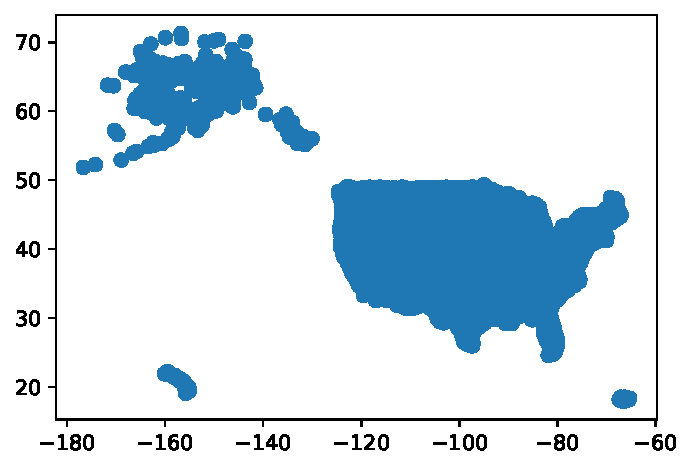
\includegraphics{pset4_template_files/figure-pdf/cell-17-output-1.pdf}

The choropleth map visually represents the distance to the nearest
hospital for each ZIP code in Texas, showing regions with greater or
lesser hospital access.

\subsection{Effects of closures on access in Texas (15
pts)}\label{effects-of-closures-on-access-in-texas-15-pts}

\begin{enumerate}
\def\labelenumi{\arabic{enumi}.}
\tightlist
\item
\end{enumerate}

\begin{Shaded}
\begin{Highlighting}[]
\CommentTok{\# Filter for Texas ZIP codes in the range 75000 to 79999 and for closures between 2016 and 2019}
\NormalTok{texas\_closures }\OperatorTok{=}\NormalTok{ corrected\_closures[}
\NormalTok{    (corrected\_closures[}\StringTok{\textquotesingle{}ZIP Code\textquotesingle{}}\NormalTok{].astype(}\BuiltInTok{str}\NormalTok{).}\BuiltInTok{str}\NormalTok{.startswith(}\BuiltInTok{tuple}\NormalTok{(}\BuiltInTok{map}\NormalTok{(}\BuiltInTok{str}\NormalTok{, }\BuiltInTok{range}\NormalTok{(}\DecValTok{750}\NormalTok{, }\DecValTok{799}\NormalTok{))))) }\OperatorTok{\&} 
\NormalTok{    (corrected\_closures[}\StringTok{\textquotesingle{}Year Closed\textquotesingle{}}\NormalTok{].between(}\StringTok{"2016"}\NormalTok{, }\StringTok{"2019"}\NormalTok{))}
\NormalTok{]}

\CommentTok{\# Group by ZIP Code and count the number of closures for each ZIP code}
\NormalTok{closures\_by\_zipcode }\OperatorTok{=}\NormalTok{ texas\_closures.groupby(}\StringTok{\textquotesingle{}ZIP Code\textquotesingle{}}\NormalTok{).size().reset\_index(name}\OperatorTok{=}\StringTok{\textquotesingle{}Number of Closures\textquotesingle{}}\NormalTok{)}

\CommentTok{\# Display the result}
\NormalTok{closures\_by\_zipcode}
\end{Highlighting}
\end{Shaded}

\begin{longtable}[]{@{}lll@{}}
\toprule\noalign{}
& ZIP Code & Number of Closures \\
\midrule\noalign{}
\endhead
\bottomrule\noalign{}
\endlastfoot
0 & 75042 & 1 \\
1 & 75231 & 1 \\
2 & 75662 & 1 \\
3 & 75862 & 1 \\
4 & 76502 & 1 \\
5 & 77035 & 1 \\
6 & 77054 & 1 \\
7 & 77429 & 1 \\
8 & 77479 & 1 \\
9 & 77598 & 1 \\
10 & 78017 & 1 \\
11 & 78061 & 1 \\
12 & 785 & 1 \\
13 & 78734 & 1 \\
14 & 78834 & 1 \\
15 & 79553 & 1 \\
16 & 79735 & 1 \\
17 & 79761 & 1 \\
\end{longtable}

\begin{enumerate}
\def\labelenumi{\arabic{enumi}.}
\setcounter{enumi}{1}
\tightlist
\item
\end{enumerate}

\begin{Shaded}
\begin{Highlighting}[]
\ImportTok{import}\NormalTok{ geopandas }\ImportTok{as}\NormalTok{ gpd}
\ImportTok{import}\NormalTok{ matplotlib.pyplot }\ImportTok{as}\NormalTok{ plt}

\CommentTok{\# Load the ZIP code shapefile}
\NormalTok{zip\_shapefile }\OperatorTok{=}\NormalTok{ gpd.read\_file(}\StringTok{\textquotesingle{}gz\_2010\_us\_860\_00\_500k/gz\_2010\_us\_860\_00\_500k.shp\textquotesingle{}}\NormalTok{)}

\CommentTok{\# Filter for Texas ZIP codes (ZIP codes starting with 750{-}799)}
\NormalTok{zip\_shapefile }\OperatorTok{=}\NormalTok{ zip\_shapefile[zip\_shapefile[}\StringTok{\textquotesingle{}ZCTA5\textquotesingle{}}\NormalTok{].}\BuiltInTok{str}\NormalTok{.startswith(}\BuiltInTok{tuple}\NormalTok{(}\BuiltInTok{map}\NormalTok{(}\BuiltInTok{str}\NormalTok{, }\BuiltInTok{range}\NormalTok{(}\DecValTok{750}\NormalTok{, }\DecValTok{800}\NormalTok{))))]}

\CommentTok{\# Ensure ZIP code columns are strings for matching}
\NormalTok{zip\_shapefile[}\StringTok{\textquotesingle{}ZCTA5\textquotesingle{}}\NormalTok{] }\OperatorTok{=}\NormalTok{ zip\_shapefile[}\StringTok{\textquotesingle{}ZCTA5\textquotesingle{}}\NormalTok{].astype(}\BuiltInTok{str}\NormalTok{)}
\NormalTok{closures\_by\_zipcode[}\StringTok{\textquotesingle{}ZIP Code\textquotesingle{}}\NormalTok{] }\OperatorTok{=}\NormalTok{ closures\_by\_zipcode[}\StringTok{\textquotesingle{}ZIP Code\textquotesingle{}}\NormalTok{].astype(}\BuiltInTok{str}\NormalTok{)}

\CommentTok{\# Merge the shapefile with closures data on ZIP code}
\NormalTok{texas\_zip\_closures }\OperatorTok{=}\NormalTok{ zip\_shapefile.merge(closures\_by\_zipcode, left\_on}\OperatorTok{=}\StringTok{\textquotesingle{}ZCTA5\textquotesingle{}}\NormalTok{, right\_on}\OperatorTok{=}\StringTok{\textquotesingle{}ZIP Code\textquotesingle{}}\NormalTok{, how}\OperatorTok{=}\StringTok{\textquotesingle{}left\textquotesingle{}}\NormalTok{)}

\CommentTok{\# Replace NaN values in \textquotesingle{}Number of Closures\textquotesingle{} with 0 for ZIP codes without closures}
\NormalTok{texas\_zip\_closures[}\StringTok{\textquotesingle{}Number of Closures\textquotesingle{}}\NormalTok{] }\OperatorTok{=}\NormalTok{ texas\_zip\_closures[}\StringTok{\textquotesingle{}Number of Closures\textquotesingle{}}\NormalTok{].fillna(}\DecValTok{0}\NormalTok{)}

\CommentTok{\# Count the number of directly affected ZIP codes (where Number of Closures \textgreater{} 0)}
\NormalTok{affected\_zip\_count }\OperatorTok{=}\NormalTok{ texas\_zip\_closures[texas\_zip\_closures[}\StringTok{\textquotesingle{}Number of Closures\textquotesingle{}}\NormalTok{] }\OperatorTok{\textgreater{}} \DecValTok{0}\NormalTok{].shape[}\DecValTok{0}\NormalTok{]}
\BuiltInTok{print}\NormalTok{(}\SpecialStringTok{f"Number of directly affected ZIP codes in Texas: }\SpecialCharTok{\{}\NormalTok{affected\_zip\_count}\SpecialCharTok{\}}\SpecialStringTok{"}\NormalTok{)}

\CommentTok{\# Plot the choropleth map}
\NormalTok{fig, ax }\OperatorTok{=}\NormalTok{ plt.subplots(}\DecValTok{1}\NormalTok{, }\DecValTok{1}\NormalTok{, figsize}\OperatorTok{=}\NormalTok{(}\DecValTok{10}\NormalTok{, }\DecValTok{10}\NormalTok{))}
\NormalTok{texas\_zip\_closures.plot(column}\OperatorTok{=}\StringTok{\textquotesingle{}Number of Closures\textquotesingle{}}\NormalTok{, cmap}\OperatorTok{=}\StringTok{\textquotesingle{}YlGnBu\textquotesingle{}}\NormalTok{, linewidth}\OperatorTok{=}\FloatTok{0.8}\NormalTok{, ax}\OperatorTok{=}\NormalTok{ax, edgecolor}\OperatorTok{=}\StringTok{\textquotesingle{}0.8\textquotesingle{}}\NormalTok{, legend}\OperatorTok{=}\VariableTok{True}\NormalTok{)}
\NormalTok{ax.set\_title(}\StringTok{\textquotesingle{}Texas ZIP Codes Directly Affected by Hospital Closures (2016{-}2019)\textquotesingle{}}\NormalTok{)}
\NormalTok{ax.set\_axis\_off()}
\NormalTok{plt.show()}
\end{Highlighting}
\end{Shaded}

\begin{verbatim}
Number of directly affected ZIP codes in Texas: 17
\end{verbatim}

\includegraphics{pset4_template_files/figure-pdf/cell-19-output-2.pdf}

\begin{enumerate}
\def\labelenumi{\arabic{enumi}.}
\setcounter{enumi}{2}
\tightlist
\item
\item
\end{enumerate}

\subsection{Reflecting on the exercise (10
pts)}\label{reflecting-on-the-exercise-10-pts}




\end{document}
